\documentclass{article}
%\documentclass[review]{elsarticle}
\usepackage{amssymb,lineno}
\modulolinenumbers[5]
\usepackage{color}
\usepackage{authblk}
\usepackage{graphics}
\usepackage{mathrsfs}
\usepackage{amsmath,bm}
\usepackage{subfigure}
%\usepackage{caption,subcaption}
\usepackage{booktabs}
\usepackage{amsthm}
\usepackage{enumerate}
\usepackage{listings}
\usepackage{appendix}
\usepackage{setspace}
\graphicspath{{TikzFig/}{Picture/}}
\usepackage{hyperref}
%\usepackage{stackengine}
\usepackage{multirow}
\usepackage[demo]{graphicx}
\usepackage[margin=2.5cm]{geometry}
\intextsep=8pt plus 3pt minus 1pt
\definecolor{ColorMark}{rgb}{1,1,1}
\numberwithin{equation}{section}
\numberwithin{table}{section}
\bibliographystyle{elsarticle-num}
\begin{document}

\title{An exact Riemann solver for one-dimensional multi-material elastic-plastic flows with Mie-Gr\"uneisen equation of state}
\author{Li Liu$^1$, Jun-bo Cheng $^{1,*}$, Jiequan Li $^{1}$}
%\author{Li Liu$^1$, Jun-bo Cheng $^{1,*}$, Jiequan Li $^{1}$}
%\cortext[mycorrespondingauthor]{
%Correspondence to: Junbo Cheng, Institute of Applied Physics and Computational Mathematics, Beijing 100094, China. E-mail: Cheng\_junbo@iapcm.ac.cn}

\maketitle

%\address{$^1$  Institute of Applied Physics and Computational Mathematics, Beijing 100094, China }

\begin{abstract}
  The Riemann problem for one-dimensional  multi-material elastic-plastic flows with the Mie-Gr\"uneisen EOS, hypo-elastic constitutive model and  the von Mises' yielding condition is studied in this paper.  Through a detailed analysis of the Jacobian matrix and relations across different type of waves,  an exact Riemann solver is constructed with totally thirty-six possible cases of structure.  Some useful results are also obtained in the analysing, for example, the sonic speed experiences a significant jump when the material is yielding and the plastic wave is always faster than the elastic wave.  More over, an exact Riemann solver is also deduced for the half Riemann problem. A lot of examples show that, the results taken by the exact Riemann solver are in good agreement with those computed by the mumerical method.

\end{abstract}

%\begin{keyword}
%  HLLC Riemann solver, high-order cell-centered Lagrangian scheme,  WENO scheme,  hypo-elastic model, elastic-plastic flows
%\end{keyword}

%\end{frontmatter}

\section{Introduction}

In this paper, an exact Riemann solver is built for one-dimensional  multi-material elastic-plastic flows with the Mie-Gr\"uneisen EOS, hypo-elastic constitutive model \cite{wilkins1963calculation} and  the von Mises' yielding condition.

The  elastic-plastic flow  is  used to describe the deformation process of solid materials under strong dynamics loading, such as explosive or high-speed impact. The simulation of elastic-plastic flows has important application backgrounds, especially in the Implosion Dynamics weapon and Inertial Confine Fusion (ICF). The first try of simulating the elastic-plastic flows was given by  Wilkins \cite{wilkins1963calculation} in 1960s.

In the development history of hydrodynamic numerical methods, the exact Riemann solver has played a very important role {\color{red}as} it not only can give a guide and reference to the construction of approximate Riemann solvers, but also can be used to determine {\color{red}the convergence and stability of numerical schemes}. However, building the exact Riemann solver for 1D elastic-plastic flows is not that easy. Comparing with the governing equations system of 1D pure fluids, for 1D elastic-plastic flows, there are two more equations: a non-conservative constitutive equation and the von Mises yielding condition.  The non-conservative character of the constitutive equation increases the difficulty in constructing  Riemann solvers, while the von Mises yielding condition may leads to more non-linear waves in the structure of Riemann solvers. Moreover, in a general way, the equation of state(EOS) for solid materials is more complex than that for pure fluids, which directly increases the difficulty in solving the Riemann problem.

For the elastic-plastic flow with the hypo-elastic constitutive model and  the von Mises' yielding condition,  some approximate Riemann solvers\cite{gavrilyuk2008modelling,cheng2015high,cheng2016harten,liumulti}  {\color{red}have been developed recently. However, for the exact Riemann solver, the research is relatively few, and them are only considered with  simple constitutive models and simple EOSs.} For example, Garaizar \cite{garaizar1991solution} and Miller \cite{miller2004iterative} introduced  an exact Riemann solver for elastic or hyper-elastic materials, Gao and Liu \cite{gao20171d,gao2018complete} firstly considered the yielding effect and developed an exact elastic-perfectly plastic solid Riemann solver, but the EOS used by them is very simple: in the elastic state, the material derivative of pressure is the linear function of the strain rate, which means the energy equation is not necessary; in the plastic state,  a linear  "stiffened-gas" EOS was used. All these makes easily deduce the relation across a non-linear wave. Although there are many  cases considered in their works \cite{gao20171d,gao2018complete}, for every case, they can easily obtain the exact solution. But for many engineering problems, the EOS is more complex, and the energy equation has to be included during simulating. For these engineering solid problems with a complex constitutive and a complex EOS, such as the Mie-Gr\"uneisen EOS, up to now, there is no  exact Riemann solution.

%Although the control equations of elastic-plastic flow is similar to the equations in computational fluid dynamics (CFD). But there are mainly three difficulties  of constructing  Riemann solvers in elastic-plastic flows.  Firstly, the constitutive models used in elastic-plastic flows are more complicated. Secondly, the EOS for solid materials is also with more characters. Finally, the yielding process of materials may lead to more wave structures.

%Recently, a lot of works have been done in constructing  approximate Riemann solvers for elastic-plastic flows with the considering of structures in the Riemann problem.  For example, Gavrilyuk et al. \cite{gavrilyuk2008modelling} analyzed the structure of the Riemann solution and constructed a Riemann solver for the linear elastic system  of hyperbolic non-conservative models for transverse waves.   Cheng et al. \cite{cheng2015high} analyzed the wave structures of one-dimensional elastic-plastic flows and developed an effective two-rarefaction approximate Riemann solver with elastic waves (TRRSE). In \cite{cheng2016harten}, for one-dimensional elastic-plastic flows, Cheng introduced a HLLCE Riemann solver, which is fast and efficient in resolving elastic waves and plastic waves. Then in \cite{liumulti}, Liu et.al remove the unreasonable assumption in HLLCE which may cause numerical errors in simulating multi-material problems and construct a multi-material HLLC elastic-plastic (MHLLCEP) solver.

%As everyone knows, in hydrodynamic numerical system, the exact Riemann solver is developed before approximate Riemann solvers \cite{godunov1959difference}, and it gives a guide and reference to the developing of approximate solvers. However, in the elastic-plastic flows, for its complexity, there are only a few works have been done in constructing the exact Riemann solver.


 %designed an exact Riemann solution of isotropic hyper-elastic material theoretically; Miller \cite{miller2004iterative} presented a general iterative method for the solution of the Riemann problem for hyperbolic elastic systems.
% Gao and Liu \cite{gao20171d,gao2018complete} firstly considered the yielding condition in, and proposed an exact elastic-perfectly plastic solid Riemann solver with both elastic and plastic states. As many as thirty-six \cite{gao20171d} and sixty-four \cite{gao2018complete} different solution types are considered in their works.
%However, in their papers,  a linear  "stiffened-gas" EOS was used in the plastic state and a more simple linear relation of pressure and strain rate is used in the elastic state. This simplification can truly deduce to simple relations  across the shock wave and rarefaction wave, but we still need an exact Riemann solver with a uniform and more common used EOS and equations system for different elastic-plastic materials. But for the elastic-plastic flows with hypo-elastic constitutive model, von Mises yielding condition and the complex equation of system(EOS), there is no exact Riemann solver. Of course, for some

%For example, Garaizar \cite{garaizar1991solution} designed an exact Riemann solution of isotropic hyperelastic material theoretically.  Miller \cite{miller2004iterative} presented a general iterative method for the solution of the Riemann problem for hyperbolic elastic systems. Gao and Liu \cite{gao20171d,gao2018complete} firstly considered the yielding condition in, and proposed an exact elastic-perfectly plastic solid Riemann solver with both elastic and plastic states. As many as thirty-six \cite{gao20171d} and sixty-four \cite{gao2018complete} different solution types are considered in their works. However, in their papers,  a linear  "stiffened-gas" EOS was used in the plastic state and a more simple linear relation of pressure and strain rate is used in the elastic state. This simplification can truly deduce to simple relations  across the shock wave and rarefaction wave, but we still need an exact Riemann solver with a uniform and more common used EOS and equations system for different elastic-plastic materials.

In this paper, we want to construct an exact Riemann solver for the system of 1D elastic-plastic flows with the Mie-Gr\"uneisen EOS, the hypo-elastic constitutive model and the von Mises' yielding condition. As every knows, the Mie-Gr\"uneisen EOS is complex and is used widely  in many engineering problems, which makes the energy equation must be included in the system of elastic-plastic flows and so we have to use some special methods to resolve the rarefaction wave. Otherwise, we analyse the Jacobian matrix and find, in the wave structures of Riemann solvers, there may be three to five waves, including one contact wave and other two to four non-linear waves. These nonlinear waves may be elastic shock waves, elastic rarefaction waves,  plastic shock waves or plastic rarefaction waves. Moreover, elastic wave runs always faster than the followed plastic wave. So there are thirty-six possible cases of the wave structures in the Riemann solver.
%For a given case, we will obtain theoretical relations of all the states as functions of density. At last,  through an iteration process of densities at both sides of the contact wave, the  exact solution will be obtained. Also, the half Riemann problem and its exact solution are considered in this paper.

%the Mie-Gr\"uneisen EOS is used for both the elastic state and plastic state of the material, which is an adequate approximation to a wide variety of materials of interest, includes some gaseous or solid explosives and solid metals under high pressure \ref{ shyue2001fluid}.  According to both the theoretical analysation and numerical tests \cite{xiao1996numerical}, in this system, there may be three to five waves, including one contact wave and elastic wave (shock or rarefaction wave) or plastic wave or both the elastic and plastic waves in each side of the contact wave. We will prove this, the elastic wave always faster than the plastic wave of  one side, so varying from the initial condition, there are $6\times 6$ thirty-six possible cases of the structures in the solution. For a given case, we will obtain theoretical relations of all the states as functions of density. At last,  through an iteration process of densities at both sides of the contact wave, the  exact solution will be obtained. Also, the half Riemann problem and its exact solution are considered in this paper.

This paper is organized as follows. In section 2, we introduce the governing equations to be studied. In section 3, the Riemann problem and the relations for every wave type (contact wave, shock wave and rarefaction wave) are  derived.  Then,  the exact Riemann solver  is given in section 4. The half Riemann problem and its solver is introduced in section 5.  Some numerical examples are presented to validate the method in section 6.  Conclusions are shown in section 7.

\section{Governing equations}
In this paper, the elastic energy is not included in the total energy. The exclution of the elastic energy is usual for practical engineering problems \cite{maire2013nominally} and is different from that in Ref.\cite{gavrilyuk2008modelling}.

%%The governing equations system is given as
%% \begin{equation}\label{eq:1d}
%   \left\{ \begin{aligned}
%       & \partial _t \rho +\partial_x(\rho u)=0,\\
%       & \partial _t (\rho u)+\partial_x(\rho u^2 + p -s_{xx})=0,\\
%       &\partial _t (\rho E)+\partial_x\left[(\rho E + p -s_{xx})u\right]=0,\\
%       &\partial _t s_{xx}+u\partial_xs_{xx}-\frac{4}{3}\partial_x u=0,\\
%& |s_{xx}|\leq \frac{2}{3}Y_{0}, \\
%        \end{aligned}
%  \right.
%\end{equation}
%It contains the following parts.
\subsection{Motion equations}
For  a continuous one-dimensional homogeneous solid, the motion equations  in differential form are
\begin{equation*}
\partial_t \mathbf{{U}} + \partial _x \bm{F}(\mathbf{{U}}) = 0, \   x \in \   \Omega \subset \mathbf{R}, \  t>0,
\end{equation*}
where
\begin{equation}
  \mathbf{U} = \left[ \begin{array}{l}
      \rho \\
      \rho u \\
      \rho  E \\
    \end{array}
  \right],
  \hspace{0.3cm}
  \mathbf{F} = \left[ \begin{array}{l}
      \rho u \\
      \rho u^2 -\sigma\\
      (\rho E -\sigma)u\\
  \end{array} \right],
\end{equation}
$\rho$, $u$, $\sigma$ and $E$ are  the density, velocity in $x-$direction, Cauchy stress and total energy per unit volume, respectively, $E$ has the relation with specific internal energy $e$ as
\begin{equation} \label{te1}
  E = e+\frac{1}{2}u^2,
\end{equation}
\begin{equation}\label{sigma1}
  \sigma = -p +s_{xx},
\end{equation}
where $p$ and $s_{xx}$ denote hydrostatic pressure and deviatoric stress in the $x-$ direction, respectively.

\subsection{The equation of state (EOS)}

The relation of the pressure with  the density and the specific internal energy is gotten from the equation of state (EOS). In this paper, we consider the Mie-Gr\"uneisen EOS,
\begin{equation}\label{eq:mie}
  p(\rho,e) = \rho_0 a_0^2f(\eta)+ \rho_0 \Gamma_0 e,
\end{equation}
where $f(\eta) = \frac{(\eta-1)(\eta-\Gamma_0(\eta-1)/2)}{(\eta-s(\eta-1))^2}$, $\eta = \frac{\rho}{\rho_0}$, $\rho_0$, $a_0$, $s$ and $\Gamma_0$ are constant parameters of the Mie-Gr\"uneisen EOS.

\subsection{The constitutive relation}
Hooke's law is used here to describe the relationship between the deviatoric stress and the strain,
\begin{equation}\label{eq:sxx1}
\dot{s}_{xx} = 2\mu \left(\dot{\varepsilon}_x-\frac{1}{3}\frac{\dot{V}}{V}\right),
\end{equation}
where $\mu$ is the shear modulus, $V$ is the volume, and the dot means the material time derivative,
\begin{equation}\label{eq:mt}
  \dot{()} = \frac{\partial ()}{\partial t} + u \frac{\partial ()}{\partial t},
\end{equation}
and
\begin{equation}\label{eq:vare}
  \dot{\varepsilon}_x = \frac{\partial u}{\partial x}, \hspace{0.3cm} \frac{\dot{V}}{V} = \frac{\partial u}{\partial x}.
\end{equation}

By using Eq.(\ref{eq:vare}), Eq.(\ref{eq:sxx1}) can be rewritten as
\begin{equation}\label{eq:sxx}
  \frac{\partial s_{xx}}{\partial t} + u \frac{\partial s_{xx}}{\partial t} =\frac{4}{3}\mu \frac{\partial u}{\partial x}.
\end{equation}

\subsection{The yielding condition}
The Von Mises' yielding condition is used here to describe the elastic limit. In one spatial dimension, the von Mises' yielding criterion is given by
\begin{equation}
  |s_{xx}| \le \frac{2}{3}Y_0,
\end{equation}
where $Y_0$ is the yield strength of the material in simple tension.

\section{The Riemann problem}\label{sec:Riemann}


The Riemann problem for the 1D time dependent elastic-plastic equations is given as follows:
 \begin{equation}\label{eq:1d}
   \left\{ \begin{aligned}
       & \partial _t \rho +\partial_x(\rho u)=0,\\
       & \partial _t (\rho u)+\partial_x(\rho u^2 + p -s_{xx})=0,\\
       &\partial _t (\rho E)+\partial_x\left[(\rho E + p -s_{xx})u\right]=0,\\
       &\partial _t s_{xx}+u\partial_xs_{xx}-\frac{4}{3}\partial_x u=0,\\
& |s_{xx}|\leq \frac{2}{3}Y_{0}, \\
       &Q(x,t = 0) = \left\{\begin{aligned}
           Q_L, \hspace{0.1cm} \text{if} \hspace{0.1cm} x<0, \\
           Q_R, \hspace{0.1cm} \text{if} \hspace{0.1cm} x\ge 0, \\
       \end{aligned}\right.
     \end{aligned}
  \right.
\end{equation}
where $Q = (\rho, \rho u, \rho E, s_{xx})^T$.


The above equations are just for the elastic status of the solid material.
If the material are in the plastic state, the above equations can be simplified
and correspondingly the jacobian matrix and sonic velocity are different.
We will discuss them separately.
\subsection{Elastic state}
\subsubsection{Jacobian matrix in elastic regions} %and the eigenvalues and eigenvectors}
For the Mie-Gr\"uneisen EOS, if the material is not yielding,
\begin{equation}
  |s_{xx}| < \frac{2}{3}Y_0,
\end{equation}
the system (\ref{eq:1d}) can be written as
\begin{equation}
 \partial_t \mathbf{Q} +\mathbf{J}_{e}(\mathbf{{Q}})\partial_x\mathbf{Q} = 0,
\end{equation}
where $Q = (\rho, \rho u, \rho E, s_{xx})$, and the Jacobian matrix is
\begin{equation}\label{eq:Jcb}
  \mathbf{J}_{e}(Q) = \left[\begin{array}{llll}
      0 & 1 & 0 & 0 \\
      -u^2 + \frac{\partial p}{\partial \rho} +\Gamma(\frac{u^2}{2}-e)& u(2-\Gamma)& \Gamma & -1 \\
	  (\Gamma(\frac{u^2}{2}-e)-e-\frac{u^2}{2}+\frac{\sigma}{\rho}+\frac{\partial p}{\partial \rho})u & -\Gamma u^2 -\frac{\sigma}{\rho}+\frac{u^2}{2} +e & (1+\Gamma)u& -u\\
    \frac{4}{3}\mu\frac{u}{\rho} & -\frac{4}{3}\mu\frac{1}{\rho}& 0 & u \\
\end{array}
\right],
\end{equation}
where $\Gamma = \frac{\Gamma_0\rho_0}{\rho} $.

The eigenvalues of $\mathbf{J}_{e}(\mathbf{Q})$ are given as
\begin{equation}
  \lambda_1 =\lambda_2 = u, \hspace{0.3cm} \lambda_3 = u-c_{e}, \hspace{0.3cm} \lambda_4 = u+c_{e},
\end{equation}
where $c_e$ means the sonic speed of the solid in the elastic state,
\begin{equation}\label{eq:c_e}
  \left\{ \begin{aligned}
      & c_e = \sqrt{a^2-\frac{\rho_0}{\rho^2}\Gamma_0 s_{xx} +\frac{4}{3}\frac{\mu}{\rho}},\\
    &   a^2 = \frac{\partial p}{\partial \rho} + \frac{p}{\rho^2}\frac{\partial p}{\partial e} = a^2_0 \frac{\partial f}{\partial \eta} + \frac{p}{\rho^2}\rho_0 \Gamma_0.
      \end{aligned} \right.
    \end{equation}
The corresponding right eigenvectors are
\begin{equation}\label{eq:eiv}
  r_1 = \left[ \begin{array}{l}
      \frac{1}{b_1} \\
      \frac{u}{b_1} \\
      0 \\
      1 \\
    \end{array}
    \right], \hspace{0.2cm}
    r_2= \left[ \begin{array}{l}
        -\frac{\Gamma}{b_1} \\
        -\frac{\Gamma u}{b_1} \\
        1 \\
        0\\
      \end{array}
    \right], \hspace{0.2cm}
r_3 =   \frac{1}{\phi^2}\left[\begin{array}{l}
        1 \\
        u-c_e \\
        h -uc_e \\
        \phi^2
      \end{array}
    \right], \hspace{0.2cm}
r_4 = \frac{1}{\phi^2}\left[\begin{array}{l}
        1 \\
        u+c_e \\
        h +uc_e \\
        \phi^2
      \end{array}
    \right],
  \end{equation}
  where
  \begin{equation}
    b_1 = \frac{\partial p}{\partial \rho} - \Gamma E,  \quad h = E +\frac{p-s_{xx}}{\rho},
  \end{equation}
  and
  \begin{equation}
    \phi^2 = a^2 -\frac{\rho_0}{\rho^2} \Gamma_0 s_{xx}-c_e^2 = -\frac{4\mu}{3}\frac{1}{\rho}.
  \end{equation}

\subsubsection{A relation between $\rho$ and $s_{xx}$ }

Thanks to (\ref{eq:mt}), the equations of the density and the deviatoric stress in Eq.(\ref{eq:1d}) can be written as
  \begin{equation}\label{eq:d1}
    \frac{\partial u}{\partial x} = -\frac{1}{\rho}\frac{d\rho}{dt},
  \end{equation}
  and
  \begin{equation}\label{eq:s1}
    \frac{ds_{xx}}{dt}=\frac{4}{3}\mu\frac{\partial u}{\partial x}.
  \end{equation}

  Substituting (\ref{eq:d1}) into (\ref{eq:s1}) yields
%  We can get a relation of density and deviatoric stress,
  \begin{equation}
    \frac{ds_{xx}}{dt}=-\frac{4}{3}\mu \frac{1}{\rho}\frac{d\rho}{dt}.
\end{equation}
Integrate the above equation from the data in front of a wave to the data behind the wave and perform some simple algebraic manipulations, one can get
\begin{equation}\label{eq:rhosxx}
  s_{xx}+\frac{4}{3}\mu\text{ln}(\rho) = \text{constant}
\end{equation}
This relation always hold in the elastic state.

\subsubsection{Relations across the contact wave}\label{sec:contacte}
  For  a  system without molecular diffusion, there is no materials convecting  across the contact wave or interface, so the velocities on two sides of  the discontinuity are always equal. % .
  This can also be verified by the eigenvectors  in Eq.(\ref{eq:eiv}) and  Eq.(\ref{eq:eivp}).

Using $\mathbf{Q}_L^*$ and $\mathbf{Q}_R^*$ to denote the two data states connected the contact wave, where $\mathbf{Q}=\left(\rho,u,p,s_{xx}\right)$.


Thanks to Eq.(\ref{eq:eiv}), for the $\lambda_{1}$-wave we
have
\begin{equation}   \label{e23a}
\frac{d \rho}{\frac{1}{b_{1}}} = \frac{d \rho u}{\frac{u
}{b_{1}}}=\frac{d \rho E}{0} = \frac{d s_{xx}}{1}.
\end{equation}
From the above equations, we can easily deduce that
\begin{equation}   \label{e23b}
du = 0, \quad d(s_{xx}-p)=0,
\end{equation}
 which means
\begin{equation}   \label{e23c}
  u_{L}^{\ast}=u_{R}^{\ast},
\end{equation}
and
\begin{equation}   \label{e23d}
\sigma_{x,L}^{\ast}=\sigma_{x,R}^{\ast},
\end{equation}
where $()_{L}^{\ast}$ and $()_{R}^{\ast}$ denote $()$ in the region
of $\mathbf{Q}_{L}^{\ast}$ and $\mathbf{Q}_{R}^{\ast}$,
respectively. Here we do not show the details of the derivation for a simple
 presentation.


Similarly, for the $\lambda_{2}$-wave one
has
\begin{equation}   \label{e24a}
\frac{d \rho}{\frac{-\Gamma}{b_{1}}} = \frac{d \rho u}{\frac{-u
\Gamma}{b_{1}}}=\frac{d \rho E}{1} = \frac{d s_{xx}}{0}.
\end{equation}
From the above equations, we can easily deduce  that
\begin{equation}   \label{e24b}
du = 0, \quad dp=0, \quad ds_{xx}=0,
\end{equation}
 which means
\begin{equation}   \label{e24c}
  u_{L}^{\ast}=u_{R}^{\ast},
\end{equation}
\begin{equation}   \label{e24d}
p_{L}^{\ast}=p_{R}^{\ast}, \quad
  s_{xx,L}^{\ast}=s_{xx,R}^{\ast}.
\end{equation}

%where $()_{L}^{\ast}$ and $()_{R}^{\ast}$ denote $()$ in the region
%of $\mathbf{W}_{L}^{\ast}$ and $\mathbf{W}_{R}^{\ast}$,
%respectively.

From  Eq.(\ref{e24d}), we  get that
\begin{equation}   \label{e27a}
\sigma_{x,L} ^{\ast}=  \sigma_{x,R} ^{\ast}.
\end{equation}


At last, for the $\lambda_{1}$ and $\lambda_{2}$ waves, one can find
that the following two relations always hold:
\begin{equation}   \label{e28}
u_{L}^{\ast}=u_{R}^{\ast}, \quad
\sigma_{x,L}^{\ast}=\sigma_{x,R}^{\ast}.
\end{equation}
For convenience, we define
\begin{equation}\label{eq:contact}
  s^* = u_L^* = u_R^*. % \hspace{0.3cm} \sigma_L^* = \sigma_R^*,
\end{equation}
where $s^*$ denotes the velocity of the contact wave.

\subsubsection{Relations across rarefaction waves}\label{sec:rarefaction}
%as an example, the state in front of the wave is known as  $(\rho_1,u_1,p_1,s_{xx1})$ and after the wave the state changes to $(\rho_2,u_2,p_2,s_{xx2})$ which is unknown.

\emph{\textbf{Left-going rarefaction wave} }
Across the left wave associated with $\lambda_3$-wave, ($\lambda_3=u-c_e$), we have
\begin{equation}
  \frac{d\rho}{1} = \frac{d(\rho u)}{u-c_e} = \frac{d(\rho E)}{h-uc_e} = \frac{ds_{xx}}{-\frac{4\mu}{3}\frac{1}{\rho}}.
\end{equation}
which leads to
\begin{align}
  \label{eq:urho}
  & \text{d} u =-\frac{c_e}{\rho}\text{d}\rho,\\
 \label{eq:Erho}
  & \text{d} E = -\frac{\sigma+\rho u c_e}{\rho^2} d\rho,\\
\label{eq:sxxrho}
& \text{d} s_{xx} = -\frac{4}{3}\frac{\mu}{\rho} d\rho.
\end{align}

Using (\ref{eq:mie}), one can get
\begin{equation}\label{te2}
  dE=de+udu.
\end{equation}

Substituting (\ref{eq:urho}) and (\ref{eq:Erho}) into the above equation yields
\begin{equation}\label{te2}
  d e = -\frac{\sigma}{\rho^2} d\rho=\frac{p-s_{xx}}{\rho^2} d\rho.
\end{equation}

Thanks to (\ref{eq:mie}), one can get
\begin{equation}\label{dp1}
  dp =  \frac{\partial p}{\partial \rho}d \rho +  \frac{\partial p}{\partial e}d e= a_0^2 \frac{\partial f}{\partial \eta} d \rho + \rho_0 \Gamma_0 de,
\end{equation}

Substituting (\ref{te2}) into the above equation yields
\begin{equation}
  dp =  \left( a_0^2 \frac{\partial f}{\partial \eta} + \frac{p}{\rho^2}\rho_0\Gamma_0 -\frac{\rho_0}{\rho^2}\Gamma_0 s_{xx}\right) d\rho.
\end{equation}

The above equation  can  be rewritten as a differential equation of $p(\rho)$
\begin{equation} \label{dp2}
  p'(\rho) - \lambda \frac{p}{\rho^2} = f_2(\rho),
\end{equation}
where
\begin{equation}
  \lambda = \rho_0 \Gamma_0 \quad f_2(\rho) = a_0^2\frac{\partial f}{\partial \eta}- \lambda\frac{s_{xx}(\rho)}{\rho^2}.
\end{equation}
By integrating (\ref{dp2}) across the left rarefaction wave, the pressure can be solved out as
\begin{equation}\label{eq:prhoEL}
  p e^{\frac{\lambda}{\rho}} - \int f_2(\rho) e^{\frac{\lambda}{\rho}}d\rho = \text{constant}.
\end{equation}
%Then for a given density $\rho$, we can get  the sonic speed $c_e$  and velocity
Integrating  (\ref{eq:urho}) across the left rarefaction wave yields
\begin{equation}\label{eq:urhoEL}
  u+\int\frac{c_e}{\rho} d\rho = \text{constant}.
\end{equation}

\emph{\textbf{Right-going rarefaction wave} }

Across the right wave associated with $\lambda_4$-wave, ($\lambda_3=u+c_e$), we have
\begin{equation}
  \frac{d\rho}{1} = \frac{d(\rho u)}{u+c_e} = \frac{d(\rho E)}{h+uc_e} = \frac{ds_{xx}}{-\frac{4\mu}{3}\frac{1}{\rho}}.
\end{equation}
which leads to
\begin{align}
  \label{eq:urhoR}
  & \text{d} u =\frac{c_e}{\rho}\text{d}\rho,\\
 \label{eq:ErhoR}
  & \text{d} E = -\frac{\sigma+\rho u c_e}{\rho^2} d\rho,\\
\label{eq:sxxrhoR}
& \text{d} s_{xx} = -\frac{4}{3}\frac{\mu}{\rho} d\rho.
\end{align}

By using the same method, one can get
\begin{equation}\label{eq:prhoER}
  p e^{\frac{\lambda}{\rho}} - \int f_2(\rho) e^{\frac{\lambda}{\rho}}d\rho = \text{constant}.
\end{equation}
\begin{equation}\label{eq:urhoER}
  u-\int\frac{c_e}{\rho} d\rho = \text{constant}.
\end{equation}

\subsubsection{Relations across  shock waves}\label{sec:shock}
Now we consider a shock wave moving with the speed of $s$. The data in front of the shock is $(\rho_1,u_1,p_1,s_{xx1})$ and that after the shock is $(\rho_2,u_2,p_2,s_{xx2})$.

%Then use the conservation relation across the wave, which is also known as the Rankine-Hugoniot relation for a shock
%\begin{align}
%  &\rho_2u_2 = \rho_1 u_1 +s(\rho_2 -\rho_1),\\
%  &\rho_2u_2^2-\sigma_{2} = \rho_1u_1^2-\sigma_{1}+s(\rho_2u_2-\rho_1u_1), \\
%  &(\rho_2E_2-\sigma_{2})u_2 = (\rho_1E_1-\sigma_{1})u_1+s(\rho_2E_2-\rho_1E_1),
%\end{align}above relations also can be written as
We transform the equations  to a frame of reference moving with the shock and the Rankine-Hugoniot Conditions give
\begin{align}
\label{eq:RH1}
  &\rho_2(u_2-s) = \rho_1(u_1-s), \\
\label{eq444}
  &\rho_2u_2(u_2-s) = \rho_1u_1(u_1-s)+\sigma_2-\sigma_1,\\
\label{eq:RH3}
  &\rho_2E_2(u_2-s) = \rho_1E_1(u_1-s)+\sigma_2 u_2-\sigma_1u_1.
\end{align}

Substituting (\ref{eq:RH1}) into (\ref{eq444}) yields
\begin{equation}\label{eq:222}
  \rho_1(u_2-u_1)(u_1-s) = \sigma_2-\sigma_1.
\end{equation}

From (\ref{eq:RH1}), one has
\begin{equation}
  u_1-s = \frac{(u_1 - u_2)\rho_2}{\rho_2 -\rho_1},
\end{equation}
then subtituting it into (\ref{eq:222}) yields
\begin{equation}\label{eq:u2u1}
  -t(u_2-u_1)^2 = \sigma_2-\sigma_1,
\end{equation}
where $ t=\frac{\rho_1 \rho_2}{\rho_2-\rho_1}$.

By using the same methods for (\ref{eq:RH3}), (\ref{eq:RH3}) can be written as
\begin{equation}
  t(u_1-u_2)(E_2-E_1) =\sigma_2 u_2-\sigma_1u_1.
\end{equation}
Because of $E= e+\frac{1}{2}u^2$, we can get
\begin{equation}\label{eq:e2e1}
  e_2 - e_1 = - \frac{\sigma_1 +\sigma_2}{2t}.
\end{equation}
Using the EOS of Mie-Gr\"uneisen (\ref{eq:mie}), can get
\begin{equation}
  e = c_0p -c_1f(\rho/\rho_0),
\end{equation}
where $c_0 = \frac{1}{\rho_0\Gamma_0}$ and $c_1 = \frac{a_0^2}{\Gamma_0}$.
Put the above equation into (\ref{eq:e2e1}), we can solve the pressure $p_2$ out as a function of $\rho_2$.
\begin{equation}\label{eq:shocke}
  p_2= \frac{2t(c_1f(\rho_2/\rho_0)+e_1)-(\sigma_1+s_{xx2})}{2tc_0-1}.
\end{equation}

Thanks to (\ref{eq:rhosxx}), $s_{xx2}$ can be written as
\begin{equation}
 s_{xx2} = s_{xx1}-\frac{4}{3}\mu\text{ln}(\frac{\rho_{2}}{\rho_{1}}).
\end{equation}

Then, the Cauchy stress can be written as
\begin{equation}
  \sigma_2 = -p_2 +s_{xx2}.
\end{equation}
Then we can use (\ref{eq:u2u1}) to solve the velocity after the shock
\begin{equation}\label{eq:shocku}
  u_2 = \left\{ \begin{aligned}
	 & u_1 - \sqrt{\frac{\sigma_1- \sigma_2}{t}} \quad \text{Left-going}, \\
	 & u_1 + \sqrt{\frac{\sigma_1- \sigma_2}{t}} \quad \text{Right-going}.
	\end{aligned}
	\right.
  \end{equation}
And the shock speed is given as
\begin{equation}
  s = \frac{\rho_2u_2-\rho_1u_1}{\rho_2-\rho_1}.
\end{equation}

By the above deductions for the moving shock wave, we can find that, if the density after the shock is known, all the data after the shock can be solved out.

\subsection{Plastic state}

When the material is yielding,
\begin{equation}\label{eq:sxxp}
  |s_{xx}| = \frac{2}{3}Y_0,
\end{equation}
the equations of Riemann problem  can be written as
\begin{equation}\label{eq:1dp}
   \left\{ \begin{aligned}
       & \partial _t \rho +\partial_x(\rho u)=0,\\
       & \partial _t (\rho u)+\partial_x(\rho u^2 + p -s_{xx})=0,\\
       &\partial _t (\rho E)+\partial_x\left[(\rho E + p -s_{xx})u\right]=0,\\
& |s_{xx}| = \frac{2}{3}Y_{0}, \\
       &U(x,t = 0) = \left\{\begin{aligned}
           U_L, \hspace{0.1cm} \text{if} \hspace{0.1cm} x<0, \\
           U_R, \hspace{0.1cm} \text{if} \hspace{0.1cm} x\ge 0, \\
       \end{aligned}\right.
     \end{aligned}
  \right.
\end{equation}
where $\mathbf{U} = (\rho, \rho u, \rho E )$.
  \subsubsection{Jacobian matrix in  plastic  regions}
  %\footnote{\href{https://nbviewer.jupyter.org/github/bfly123/Exact-Elastic-plastic-Riemann-Solver-/blob/master/\%20CharacteristicForPlasticStateAfterYielding.ipynb\#}{Code site link}}}
 The motion equations of (\ref{eq:1dp}) can be written as
\begin{equation}
  \partial_t \mathbf{{U}} + \mathbf{J}_p(\mathbf{U})\partial_x \mathbf{{U}}= 0,
\end{equation}
 where the Jacobian matrix is
\begin{equation}
\mathbf{J}_p(\mathbf{U}) = \left[\begin{array}{lll}
      0 & 1 & 0   \\
      -u^2 + \frac{\partial p}{\partial \rho} +\Gamma(\frac{u^2}{2}-e)& u(2-\Gamma)& \Gamma \\
	  (\Gamma(\frac{u^2}{2}-e)-e-\frac{u^2}{2}+\frac{\sigma}{\rho}+\frac{\partial p}{\partial \rho})u +\frac{u^2}{2} & -\Gamma u^2 -\frac{\sigma}{\rho} +e & (1+\Gamma)u\\
\end{array}
\right].
\end{equation}

The eigenvalues of $\mathbf{J}_p(\mathbf{Q})$ are given as
$$\lambda_1 = u,\quad \lambda_2 = u-c_p, \quad \lambda_3 = u+c_p,$$
where
\begin{equation}\label{eq:c_p}
   c_p = \sqrt{a^2-\frac{\rho_0}{\rho^2}\Gamma_0 s_{xx}}.
\end{equation}
%\begin{equation}\label{eq:c_p}
%  \left\{ \begin{aligned}
%	  & c_p = \sqrt{a^2-\frac{\rho_0}{\rho^2}\Gamma_0 s_{xx}} ,\\
%    &   a^2 = \frac{\partial p}{\partial \rho} + \frac{p}{\rho^2}\frac{\partial p}{\partial e} = a^2_0 \frac{\partial f}{\partial \eta} + \frac{p}{\rho^2}\rho_0 \Gamma_0.
%      \end{aligned} \right.
%    \end{equation}
The corresponding right eigenvectors are
\begin{equation}\label{eq:eivp}
  r_1 = \left[ \begin{array}{l}
	  -\frac{\Gamma}{b_1} \\
	  -\frac{\Gamma u}{b_1} \\
	  1\\
  \end{array}\right], \quad
  r_2 = \frac{1}{h-uc_p} \left[  \begin{array}{l}
	  1 \\
	  u-c_p \\
	  h-uc_p\\
  \end{array}\right], \quad
 r_3 = \frac{1}{h+uc_p}\left[ \begin{array}{l}
	  1 \\
	  u+c_p \\
	  h+uc_p\\
  \end{array}\right].
\end{equation}
%where
% \begin{equation}
%    b_1 = \frac{\partial p}{\partial \rho} - \Gamma E,  \quad h = E +\frac{p-s_{xx}}{\rho}.
%  \end{equation}

Comparing Eq.(\ref{eq:c_e}) with Eq.(\ref{eq:c_p}), we notice that the sonic speed is not continuous between the states of elastic and plastic. As the shear modulus $\mu$ is always positive, so the elastic wave runs always faster than the plastic wave.  %This is very important and may cause wrong results if ignoring it.

\subsubsection{Relations across the contact wave}\label{sec:contactp}

According to  the eigenvectors in  Eq.(\ref{eq:eivp}), for the $\lambda_{1}$-wave ($\lambda_1 = u$), we
have
\begin{equation}   \label{e232a}
  \frac{d \rho}{\frac{-\Gamma}{b_1}} = \frac{d (\rho u)}{\frac{-u\Gamma}{b_1}} = \frac{d (\rho E)}{1}.
\end{equation}
From the above equations, we can easily deduce that
\begin{equation}
  du = 0, \quad dp = 0,
\end{equation}
%Samilar to that in  section \ref{sec:contacte}, we can also get the relations
which means that
\begin{equation}
u_L^* = u_R^*, % \hspace{0.3cm} \sigma_L^* = \sigma_R^*,
 \quad
  p^*_L = p^*_R.
\end{equation}
Because $s^*_{xxL} = s^*_{xxR}$, thanks to (\ref{sigma1}), one can get
\begin{equation}
  \sigma^*_L = \sigma^*_R.
\end{equation}
For convenience, we define
\begin{equation}
  s^* = u_L^* = u_R^*.
\end{equation}

\subsubsection{Relations across rarefaction waves}
%as an example, the state in front of the wave is known as  $(\rho_1,u_1,p_1,s_{xx1})$ and after the wave the state changes to $(\rho_2,u_2,p_2,s_{xx2})$ which is unknown.

\emph{\textbf{Left-going rarefaction wave} }
Across the left wave associated with $\lambda_2$-wave, ($\lambda_2=u-c_p$), we have
\begin{equation}
  \frac{d\rho}{1} = \frac{d(\rho u)}{u-c_p} = \frac{d(\rho E)}{h-uc_p}.
\end{equation}
Samilar to section \ref{sec:rarefaction}, we can get the relations
\begin{equation}\label{eq:p_rhopL}
  p e^{\frac{\lambda}{\rho}} - \int f_2(\rho) e^{\frac{\lambda}{\rho}}d\rho = \text{constant}.
\end{equation}
and
\begin{equation}\label{eq:u_rhopL}
  u+\int\frac{c_p}{\rho} d\rho = \text{constant}.
\end{equation}
%where
%\begin{equation}
%  \lambda = \rho_0 \Gamma_0 \quad f_2(\rho) = a_0^2\frac{\partial f}{\partial \eta}- \lambda\frac{s_{xx}(\rho)}{\rho^2}.
%\end{equation}

\emph{\textbf{Right-going rarefaction wave} }
Across the right wave associated with $\lambda_3$-wave, ($\lambda_3=u+c_e$), we have
\begin{equation}
  \frac{d\rho}{1} = \frac{d(\rho u)}{u+c_p} = \frac{d(\rho E)}{h+uc_p}.
\end{equation}
We can get  similar  relations  as the left-going wave as
\begin{equation}\label{eq:p_rhopR}
  p e^{\frac{\lambda}{\rho}} - \int f_2(\rho) e^{\frac{\lambda}{\rho}}d\rho = \text{constant}.
\end{equation}
\begin{equation}\label{eq:u_rhopR}
  u-\int\frac{c_p}{\rho} d\rho = \text{constant}.
\end{equation}

\subsubsection{Relations across  a shock wave}\label{sec:shockp}
By using the same deducing process as Section \ref{sec:shock}, we can get the states after the shock wave as
\begin{equation}
  s_{xx2} = s_{xx1},
\end{equation}
\begin{equation}\label{eq:shockp}
  p_2= \frac{2t(c_1f(\rho_2/\rho_0)+e_1)-(\sigma_1+s_{xx2})}{2tc_0-1},
\end{equation}
where $c_0 = \frac{1}{\rho_0\Gamma_0}$, $c_1 = \frac{a_0^2}{\Gamma_0}$, $\sigma_2 = -p_2 +s_{xx2}$,
%\begin{equation}
%  \sigma_2 = -p_2 +s_{xx2},
%\end{equation}
\begin{equation}\label{eq:shockup}
  u_2 = \left\{ \begin{aligned}
	 & u_1 - \sqrt{\frac{\sigma_1- \sigma_2}{t}} \quad \text{Left-going}, \\
	 & u_1 + \sqrt{\frac{\sigma_1- \sigma_2}{t}} \quad \text{Right-going}.
	\end{aligned}
	\right.
  \end{equation}
And the shock speed is given as
\begin{equation}
  s = \frac{\rho_2u_2-\rho_1u_1}{\rho_2-\rho_1}.
\end{equation}


\section{Exact Riemann solver} %\footnote{\href{https://nbviewer.jupyter.org/github/bfly123/Exact-Elastic-plastic-Riemann-Solver-/blob/master/\%20CharacteristicForPlasticStateAfterYielding.ipynb\#}{Code site link}}} \label{sec:riemann}

%Althoughx HLLCE Riemann solver can simulate the elastic-plastic flow effectively and efficiently without iterations, but the plastic structure is not considered in and  there are some assumptions that are not so reasonable, especially in the interface between different materials. For example, the normal stresses $\sigma_x$ are  always equavalent across the interface, but the pressures are not always equal, and the consequent evaluation of $\widetilde{s}^*$ may   be of large error.

Now we consider the constructing details of the exact  Riemann  solver. For  the Riemann problem in Section \ref{sec:riemann}, there are  $6\times 6$ possible  cases in the Riemann solution with different wave structures.  The left six cases are  shown in Fig.\ref{fig:cases}.


\begin{figure}
%\captionsetup[subfigure]{labelformat=empty}
  \centering
  \subfigure[Elastic rarefaction wave ($R^{E}$)]{
	\label{fig:subfigure:a}
  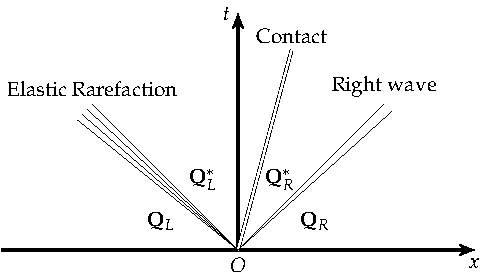
\includegraphics[width=5cm]{Tikz-figure0.eps}}
  \subfigure[Plastic rarefaction wave ($R^{P}$)]{
	\label{fig:subfigure:b}
  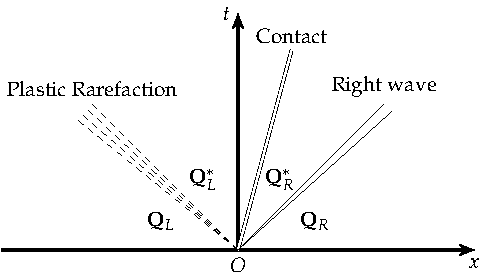
\includegraphics[width=5cm]{Tikz-figure1.eps}}
  \subfigure[Both elastic and plastic rarefaction waves ($R^{E}R^{P}$)] {
	\label{fig:subfigure:c}
  \includegraphics[width=5cm]{Tikz-figure2.eps}}
  \subfigure[ Elastic shock wave ($S^{E}$)]{
	\label{fig:subfigure:d}
  \includegraphics[width=5cm]{Tikz-figure3.eps}}
  \subfigure[Plastic shock wave ($R^{P}$) ]{
	\label{fig:subfigure:e}
  \includegraphics[width=5cm]{Tikz-figure4.eps}}
  \subfigure[Both elastic and plastic shock waves ($S^{E}S^{P}$)]{
	\label{fig:subfigure:f}
	\includegraphics[width=5cm]{Tikz-figure5.eps}}
  \caption{The possible cases of Riemann solution structures in the left side.}
  \label{fig:cases}
\end{figure}

%\begin{figure}
%  \centering
%\stackunder{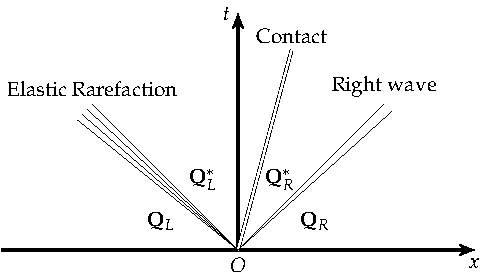
\includegraphics[width=3.6cm]{Tikz-figure0.eps}}{\tiny ($\!R^\!E\!$) Elastic rarefaction}%
%\stackunder{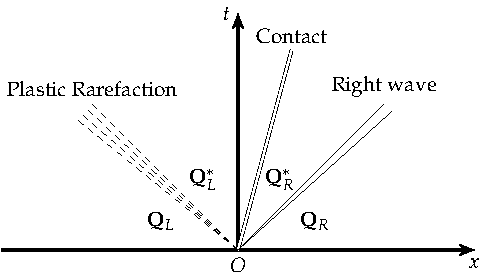
\includegraphics[width=3.6cm]{Tikz-figure1.eps}}{\tiny ($\!R^\!P\!$) Plastic rarefaction}
%\stackunder{\includegraphics[width=3.6cm]{Tikz-figure2.eps}}{\tiny ($\!R\!^E\!R\!^P\!$) Both elastic and plastic rarefactions}
%\stackunder{\includegraphics[width=3.6cm]{Tikz-figure3.eps}}{\tiny ($\!S^\!E$) Elastic shock}%
%\stackunder{\includegraphics[width=3.6cm]{Tikz-figure4.eps}}{\tiny ($\!S^\!P\!$) Plastic shock}
%\stackunder{\includegraphics[width=3.6cm]{Tikz-figure5.eps}}{\tiny ($\!S\!^E\!S\!^P\!$) Both elastic and plastic shocks}
%\caption{November to April}
%\end{figure}

%There are mainly five  steps in the soluting process.
%\begin{enumerate}
%  \item In section (\ref{sec:eva}), a pre-evaluation is done with a shock-contact-shock waves assumption to give an initial values of $\rho^*_L$ and $\rho^*_R$.
%
%  \item  With  given $\rho^*_L$ and $\rho^*_R$, we need to  detect the left cases in Fig.\ref{fig:cases} and the corresponding right cases, this is done in section \ref{sec:eva}.
%
%  \item  We solve functions $s_{xx}(\rho)$, $p(\rho)$ and $u(\rho)$ for  different cases in section \ref{sec:one}.
%
%\item At last,   with  the informations in Section \ref{sec:contact},
%\begin{equation}\label{eq:fus}
%  \begin{aligned}
%	f_u(\rho^*_L,\rho^*_R) = u_L^* -u_R^* = 0,\\
%	f_\sigma(\rho^*_L,\rho^*_R) = \sigma_L^* -\sigma_R^* = 0,
%\end{aligned}
%\end{equation}
% use a Newton iteration method to  get new $\rho^*_L$ and $\rho^*_R$, then do steps 2-5 again until the result convergents. this process is given in Section \ref{sec:iteration}.
%\end{enumerate}

  \subsection{The solving process}\label{sec:iteration}
  %From those relations in Section  \ref{sec:Riemann}, all  variables can be formulated in terms of density.
  %So, given densities in unknown regions $\mathbf{Q}^*_L$ and  $\mathbf{Q}^*_R$, the Riemann problem is solved.
From Section  \ref{sec:Riemann}, we can find that all variables can be formulated in terms of density. So we define equations
\begin{equation}
\left\{
\begin{array}{c}
  f_u(\rho_L^*,\rho_R^*,\mathbf{Q}_{L},\mathbf{Q}_{R})_=  u_L^*(\rho_L^*,\mathbf{Q}_{L}) -u_R^*(\rho_R^*,\mathbf{Q}_{R}), \\
  f_\sigma(\rho_L^*,\rho_R^*,\mathbf{Q}_{L},\mathbf{Q}_{R})_=  \sigma_L^*(\rho_L^*,\mathbf{Q}_{L}) -\sigma_R^*(\rho_R^*,\mathbf{Q}_{R}).
\end{array}
\right.
\end{equation}
By using the relations across the contact wave in Section \ref{sec:contacte} and Section \ref{sec:contactp}, we can get
\begin{equation} \label{exact1}
\left\{
\begin{array}{c}
  f_u(\rho_L^*,\rho_R^*,\mathbf{Q}_{L},\mathbf{Q}_{R})_=  u_L^*(\rho_L^*,\mathbf{Q}_{L}) -u_R^*(\rho_R^*,\mathbf{Q}_{R})=0, \\
  f_\sigma(\rho_L^*,\rho_R^*,\mathbf{Q}_{L},\mathbf{Q}_{R})_=  \sigma_L^*(\rho_L^*,\mathbf{Q}_{L}) -\sigma_R^*(\rho_R^*,\mathbf{Q}_{R})=0.
\end{array}
\right.
\end{equation}

Obviously, this system is uniquely solvable, but we can not get the analytical solution of (\ref{exact1}). We have to use an iteration procedure to solve (\ref{exact1}) and
%, which is given in the following.
%Given values of $\rho_L^*$ and  $\rho_R^*$,  by using relations across the contact wave in Section \ref{sec:contacte} and Section \ref{sec:contactp}, we can get
%\begin{equation}
%  \begin{aligned}
%	f_u(\rho_L^*,\rho_R^*)_=  u_L^* -u_R^* =0,\\
%	f_\sigma(\rho_L^*,\rho_R^*)_=  \sigma_L^* -\sigma_R^* =0.\\
%\end{aligned}
%\end{equation}
%Then using a  Newton iteration method, we can solve the densities $\rho_L^*$ and $\rho_R^*$ out.
the solving process is shown in Fig.\ref{fig:newton}. The details are introduced in the following.
\begin{figure}
  \centering
  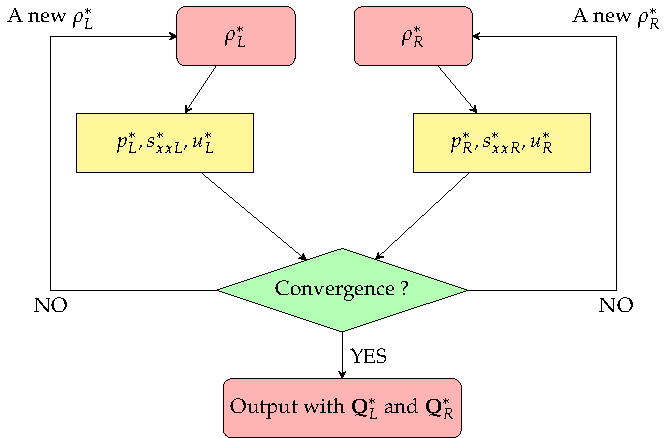
\includegraphics[width= 10cm] {Tikz-figure6.eps}
  \caption{A flow chat of the Newton iteration process.}
  \label{fig:newton}
\end{figure}


\noindent  \textbf{Initial:}

	The initial densities are given as
\begin{equation}
  \rho_{L(1)}^* = \frac{\rho_L+\rho_R}{2} \quad \rho_{R(1)}^* = \frac{\rho_L+\rho_R}{2}.
\end{equation}

\noindent
\textbf{Iteration begin:}
\begin{enumerate}[Step 1]
  \item Determining the case of the wave structure:

	Given $\rho _{L(k)}^*$ and a  $\rho _{R(k)}^*$ in the $k$-th  iteration step, we can use the methods introduced in Section \ref{sec:deter} to determine the case of wave structure of this Riemann problem. In this procedure for solving this Riemann problem, the subscript $(k)$ means the variable in the $k$-th  iteration step.

  \item Evaluating $f_{u(k)}$ and $f_{\sigma(k)}$:

  After determining the structure case, we need  to solve the Cauchy stresses and the velocities in regions $\mathbf{Q}^*_L$ and $\mathbf{Q}^*_R$, those are given in Section \ref{sec:functions}.

  \item Evaluating the derivatives of $f_{u(k)}$ and $f_{\sigma(k)}$.

The derivatives of $f_{u(k)}$ and $f_{\sigma(k)}$ are given as
\begin{equation}
  \frac{\partial f_{u(k)}}{\partial \rho^*_{L(R)}} = \frac{f_{u(k)}-f_{u(k-1)}}{\rho_{L(R)(k)}^* - \rho_{L(R)(k-1)}},\quad
  \frac{\partial f_{\sigma(k)}}{\partial \rho^*_{L(R)}} = \frac{f_{\sigma(k)}-f_{\sigma(k-1)}}{\rho_{L(R)(k)}^* - \rho_{L(R)(k-1)}}.
\end{equation}
At the first step, we use a simple  numerical difference  method
\begin{equation}
  \frac{\partial f_{u(1)}}{\partial \rho^*_{L(R)}} = \frac{f_{u}(\rho^*_{L(R)}+\Delta \rho)-f_{u}(\rho^*_{L(R)})}{\Delta \rho_{L(R)}},\quad
  \frac{\partial f_{u(1)}}{\partial \rho^*_{L(R)}} = \frac{f_{u}(\rho^*_{L(R)}+\Delta \rho)-f_{u}(\rho^*_{L(R)})}{\Delta \rho_{L(R)}},
\end{equation}
where $\Delta \rho$ is a little quantity, we define
\begin{equation}
  \Delta \rho = \frac{\rho_{L(R)(1)}^*}{100}.
\end{equation}

  \item  Evaluating  $\rho_{L(k+1)}^*$ and $\rho_{R(k+1)}^*$:
\begin{equation}
\left[ \begin{array}{l}
 \rho _{L(k+1)}^*\\
\rho_{R(k+1)}^*\\
\end{array}
\right] =
\left[ \begin{array}{l}
 \rho _{L(k)}^*\\
\rho_{R(k)}^*\\
\end{array}
\right]-
\left[ \begin{array}{ll}
\frac{\partial f_{u(k)}}{\partial \rho_L^*} & \frac{\partial f_{u(k)}}{\partial \rho_R^*}\\
\frac{\partial f_{\sigma(k)}}{\partial \rho_L^*} & \frac{\partial f_{\sigma(k)}}{\partial \rho_R^*}\\
\end{array}
\right]^{-1}
\left[ \begin{array}{l}
f_{u(k)}\\
f_{\sigma(k)}\\
\end{array}
\right]
\end{equation}

\item Convergence test:

The iteration is convergent if
\begin{equation}{\label{conv}}
  \text{CHA} \le \text{TOL},
\end{equation}
where
%The convergence is measured by
\begin{equation}
\text{CHA} = \text{max} \left[
\frac{|\rho_{L(k+1)}^*- \rho_{L,(k)}^*|}{\frac{1}{2}|\rho_{L(k+1)}^*+\rho_{L(k)}^*|},   \frac{|\rho_{R(k+1)}^*- \rho_{R,(k)}^*|}{\frac{1}{2}|\rho_{R(k+1)}^*+\rho_{R(k)}^*|},|f_{u}|,|f_{\sigma}|\right],
\end{equation}
$$\text{TOL} = 10^{-4}.$$
%and the tolerance is taken as .
If not, go to Step 1 and continue the iteration procedure until convergent. Numerical examples show, after 2-4 iterations, the condition (\ref{conv} ) is satisfied.
%It usually takes 2-4 steps to get a convergence result.
\end{enumerate}

\noindent
\textbf{Iteration end}
%\subsection{Pre-evaluation of densities}\label{sec:eva}
%At first, we assume that there are only one elastic shock wave in the left side and another one  elastic shock in the right side as shown in Fig.\ref{fig:HLLC}. According to the conservation relations across the shocks, we have
%\begin{equation}
%  \left\{
%  \begin{aligned}
%	&\hat{\rho}_L\hat{u}^*_L = \rho_L u_L +s_L(\hat{\rho}_L^*-\rho_L), \\
%	&\hat{\rho}_L\hat{u}_L^{*2}-\sigma_L^* = \rho_L u_L^2 -\sigma_L +s_L(\hat{\rho}_L^* \hat{u}_L^*-\rho_L u_L),
%  \end{aligned}
%\right.
%\end{equation}
%and
%\begin{equation}
%  \left\{
%  \begin{aligned}
%	&\hat{\rho}_R\hat{u}^*_R = \rho_R u_R +s_R(\hat{\rho}_R^*-\rho_R), \\
%	&\hat{\rho}_R\hat{u}_R^{*2}-\sigma_R^* = \rho_R u_R^2 -\sigma_R +s_R(\hat{\rho}_R^* \hat{u}_R^*-\rho_R u_R).
%  \end{aligned}
%\right.
%\end{equation}
%\begin{figure}
%  \centering
%  \includegraphics[width=8cm]{Tikz-figure7.eps}
%  \caption{Pre-evaluation with a three-waves structure.}
%  \label{fig:HLLC}
%\end{figure}
%
%
%Using the relation across the interface,
%\begin{equation}
%  \hat{u}_L^* = \hat{u}_R^* =\hat{s}^*,\quad \hat{\sigma}_L^* = \hat{\sigma}_R^*.
%\end{equation}
%the speed of contact wave can be evaluated as
%\begin{equation}
%\hat{s}^* = \frac{\sigma_L-\sigma_R+\rho_L u_L(s_L-u_L)-\rho_R u_R(s_R-u_R)}{\rho_L(s_L-u_L)-\rho_R(s_R-u_R)},
%\end{equation}
%the density is solved as
%\begin{equation}
%\hat{\rho}_L^* = \frac{\rho_L(u_L-s_L)}{\hat{s}^*-s_L}, \quad
%\hat{\rho}_R^* = \frac{\rho_R(u_R-s_R)}{\hat{s}^*-s_R}.
%\end{equation}
%Here we define the speeds of left and right going waves as
% \begin{equation}
%      s_L = \text{min} (u_L-c_L, u_R-c_R, 0),  \quad s_R = \text{max}(u_L+c_L, u_R+c_R, 0).
%\end{equation}
\subsection{Determining the case of structures} \label{sec:deter}

Given the value of density $\rho^*_{L(R)}$, we can distinguish the non-linear wave is a shock or rarefaction wave.  This is done easily by comparing $\rho^*_{L(R)}$ with $\rho_{L(R)}$, the subscript $_{L(R)}$ means in the left(right) side of the contact wave.
\begin{equation}\label{shock1}
  \left\{
  \begin{aligned}
	& \text{a rarefaction wave:} & \text{if} \ \rho_{L(R)} > \rho_{L(R)}^*,\\
	& \text{a shock wave:} &   \text{if} \ \rho_{L(R)} < \rho_{L(R)}^*.\\
\end{aligned}\right.
\end{equation}

Thanks to (\ref{eq:rhosxx}),
%To determine the number of waves, we need to know the yielding situation,
the deviatoric stress can be evaluated as
\begin{equation}  \label{sxx1}
\hat{s}_{xxL(R)}=-\frac{4}{3}\mu\text{ln}\left(\frac{\rho_{L(R)}^*}{\rho_{L(R)}}\right)+s_{xxL(R)}.
\end{equation}

According to the values of initial and evaluated deviatoric stresses in (\ref{sxx1}) in one side of the contact wave, the non-linear wave in this side may be:

{\color{red}
\begin{equation} \label{yield1}
  \left\{
  \begin{aligned}
	& \text{an elastic  rarefaction} & \text{if}  \ \hat{s}_{xxL(R)}<\frac{2}{3}Y^{0},\\
	& \text{a plastic rarefaction} & \text{if} \ {s}_{xxL(R)} = \frac{2}{3}Y^{0} \ \text{and} \ \hat{s}_{xxL(R)} \geq \frac{2}{3}Y_{0},\\
	& \text{an elastic rarefaction  and a following plastic rarefaction} &  \text{if} \ {s}_{xxL(R)} < \frac{2}{3}Y^{0} \ \text{and} \ \hat{s}_{xxL(R)} \geq \frac{2}{3}Y_{0},\\
	& \text{an elastic shock} & \text{if}  \ \hat{s}_{xxL(R)}> -\frac{2}{3}Y_{0},\\
	& \text{a plastic shock} & \text{if} \ {s}_{xxL(R)} = -\frac{2}{3}Y^{0} \ \text{and} \ \hat{s}_{xxL(R)} \leq -\frac{2}{3}Y_{0},\\
	& \text{an elastic shock and a following plastic shock} &  \text{if} \ {s}_{xxL(R)} > -\frac{2}{3}Y^{0} \ \text{and} \ \hat{s}_{xxL(R)} \leq -\frac{2}{3}Y_{0}.
\end{aligned}\right.
\end{equation}
}

Combining (\ref{shock1}) and (\ref{yield1}), we can find, in any side of the wave structure of this Riemann problem, there are six cases showed in Table \ref{tab:cases}, where capital letters ''S'' and ''R'' mean the shock and rarefaction wave, respectively; superscript letters ''E'' and  ''P'' indicate the elastic or plastic state of a wave, respectively. Otherwise, the  subscript $L$ or  $R$  are omitted for simplification.

%  Then we can classify every side into six cases, and conditions for the classfication are  shown in Table \ref{tab:cases}, the  subscripts $_L$ and  $_R$  are omitted for simplication.

{\color{red}
\begin{table}
  \centering
  \caption{The condition of  cases classification.}
  \begin{tabular}{c|ccc}
	\toprule
	\multirow{2}{*}{  $\hat{\rho^*} <\rho$ }  &  $\hat{s}_{xx}<\frac{2}{3}Y_0$ & $s_{xx}=\frac{2}{3}Y_0$ and  $\hat{s}_{xx} \geq \frac{2}{3}Y_0$ &  other\\
	\cline{2-4}
 & case a: $R^{E}$ & case b: $ R^{P}$ & case c: $R^{E}R^{P}$ \\
 \hline
 \multirow{2}{*}{  $\hat{\rho^*} >\rho$ } & $\hat{s}_{xx} > -\frac{2}{3}Y_0$ & $s_{xx}=-\frac{2}{3}Y_0$  and  $\hat{s}_{xx} \leq -\frac{2}{3}Y_0$&  other\\
	\cline{2-4}
  & case d: $S^{E}$ & case e: $ S^{P}$ & case f: $S^{E}S^{P}$ \\
  %\hline
  \bottomrule
\end{tabular}
\label{tab:cases}
\end{table}
}

\subsection{States in  middle regions ($\tilde{\mathbf{Q}}_{L}$ and   $\tilde{\mathbf{Q}}_{R}$) }


\emph{\textbf{Cases ($R^{E}$, $R^{P}$, $S^{E}$ and $S^{P}$)}}

 For cases ($R^{E}$, $R^{P}$, $S^{E}$ and $S^{P}$) in Fig.\ref{fig:cases}, the material is totally yielding or totally not yielding, there is no midlle state $\tilde{\mathbf{Q}}_{L(R)}$. For  expression convenience, we let
 \begin{equation}
   (\tilde{\rho}_{L(R)},\tilde{u}_{L(R)},\tilde{p}_{L(R)},\tilde{s}_{xx}) =(\rho_{L(R)}, u_{L(R)},p_{L(R)},s_{xxL(R)}),
\end{equation}

%For cases ($R^{E}R^{P}$, $S^{E}S^{P}$), the material will experience the process from the non-yielding condition to the yielding condition and so there are two non-linear waves in the one side of the wave structure and the middle state $\tilde{\mathbf{Q}}_{L(R)}$ exists. In the middle state $\tilde{\mathbf{Q}}_{L(R)}$, the deviatoric stress achieves the elastic limit.
%\begin{equation}
% \tilde{s}_{xxL(R)} = \left\{ \begin{aligned}
%	 &\frac{2}{3}Y_0 \quad  &\text{Case ($R^{E}R^{P}$)},\\
%	 &-\frac{2}{3}Y_0 \quad &\text{Case ($S^{E}S^{P}$)}.
%	\end{aligned}
%  \right.
%\end{equation}

%Thanks to (\ref{eq:rhosxx}),  the density in $\tilde{\mathbf{Q}}_{L(R)}$ is given as
%\begin{equation}
%  \tilde{\rho}_{L(R)}= \left\{ \begin{aligned}
%	  & \rho_{L(R)} \text{exp}\left(-\frac{Y_0}{2\mu}+\frac{3 s_{xxL(R)}}{4\mu}\right), \quad  & \text{Case ($R^{E}R^{P}$)}, \\
%	  & \rho_{L(R)} \text{exp}\left(\frac{Y_0}{2\mu}+\frac{3 s_{xxL(R)}}{4\mu}\right), \quad  & \text{Case ($S^{E}S^{P}$)}.
%	\end{aligned}
%  \right.
%	\end{equation}

	\emph{\textbf{Case ($R^{E}R^{P}$)}}

Using the methods introduced in  the Section (\ref{sec:rarefaction}), we can easily deduce the formulation of all unknown variables after the rarefaction wave. Here we do not show the details of deduction.

%For rarefaction wave case, we give the function of $s_{xx}$ at first,
%\begin{equation}
%  s_{xx}(\rho) =	 -\frac{4}{3}\mu\text{ln}\left(\frac{\rho}{\rho_{L(R)}}\right)+s_{xxL(R)} \quad  \rho_{L(R)} \ge \rho \ge \tilde{\rho}_{L(R)}
%  \end{equation}

For the case ($R^{E}R^{P}$),  after the elastic rarefaction wave, the deviatoric stress achieves the elastic limit. Thanks to (\ref{shock1}) and (\ref{yield1}), one can easily deduce that
\begin{equation*}
\tilde{s}_{xxL(R)} = \frac{2}{3}Y_0.
\end{equation*}

By using (\ref{eq:rhosxx}), the density in $\tilde{\mathbf{Q}}_{L(R)}$ is given as
\begin{equation*}
\tilde{\rho}_{L(R)} = \rho_{L(R)} \text{exp}\left(-\frac{Y_0}{2\mu}+\frac{3 s_{xxL(R)}}{4\mu}\right).
\end{equation*}

From (\ref{eq:prhoEL}) and (\ref{eq:prhoER}), for the case ($R^{E}R^{P}$), the pressure is rearranged as
\begin{equation}\label{rerpp}
  p(\rho)=
	  p_{L(R)}e^{\frac{\lambda}{\rho_{L(R)}}-\frac{\lambda}{\rho}} +e^{-\frac{\lambda}{\rho}}\int_{\rho_{L(R)}}^{\rho} f_2(x) e^{\frac{\lambda}{x}}dx, %\quad  \rho_{L(R)}\ge \rho \ge \tilde{\rho}_{L(R)},
\end{equation}
where
\begin{equation}
  \lambda = \rho_0 \Gamma_0 \quad f_2(\rho) = a_0^2\frac{\partial f}{\partial \eta}- \lambda\frac{s_{xx}(\rho)}{\rho^2}, \ s_{xx}(\rho) =	 -\frac{4}{3}\mu\text{ln}\left(\frac{\rho}{\rho_{L(R)}}\right)+s_{xxL(R)}.
\end{equation}


Thanks to (\ref{eq:urhoEL}) and (\ref{eq:urhoER}), for the rarefaction wave case ($R^{E}R^{P}$), the velocity is given as
\begin{equation} \label{rerpu}
  u(\rho) =\left\{ \begin{aligned}
	&u_L - \int_{\rho_L}^{\rho} \frac{c_e(x)}{x} dx \quad  & \text{for the  left-going rarefaction wave}
 , \\
 &u_R + \int_{\rho_R}^{\rho} \frac{c_e(x)}{x} dx \quad &  \text{for the right-going rarefaction wave} ,
	\end{aligned}
  \right. % \quad \text{case (c)}.
\end{equation}
where the sonic speed
\begin{equation}
  c_e(\rho) =
	  \sqrt{a_0^2 \frac{\partial f}{\partial \eta} + \frac{p(\rho)}{\rho^2}\rho_0\Gamma_0 -\frac{\rho_0}{\rho^2}\Gamma_0 s_{xx}(\rho) +\frac{4}{3}\frac{\mu}{\rho}}. % \quad  \rho_{L(R)} \ge \rho \ge \tilde{\rho}_{L(R)}
\end{equation}

States in region $\tilde{\mathbf{Q}}_{L(R)}$ can be solved as
\begin{equation}
  % \tilde{s}_{xxL(R)} = s_{xx}(\rho_{L(R)}),\quad
  \tilde{p}_{L(R)} = p(\rho_{L(R)}), \quad \tilde{u}_{L(R)} = u(\rho_{L(R)}).
\end{equation}

\textbf{Remark}:  In (\ref{rerpp}) and (\ref{rerpu}), there are two integral terms. Obviously, because of the complexity of the EOS, we can not get the exact integral values. We have to use the numerical methods to approximate the two integral terms with high order of accuracy. The approximation methods are introduced in the Appendix 1. 


\emph{\textbf{Case ($S^{E}S^{P}$)}}

Using the methods introduced in  the Section (\ref{sec:shock}), we can easily deduce the formulation of all unknown variables in $\tilde{\mathbf{Q}}_{L(R)}$. In order to shorten the length of our paper, we do not show the details of the deduction.

For the case ($S^{E}S^{P}$), after the elastic shock wave, the deviatoric stress achieves the elastic limit. So, by using (\ref{shock1}) and (\ref{yield1}), one can easily deduce that
\begin{equation*}
\tilde{s}_{xxL(R)} = -\frac{2}{3}Y_0.
\end{equation*}

From (\ref{eq:rhosxx}), after the elastic shock wave, the density in $\tilde{\mathbf{Q}}_{L(R)}$ is given as
\begin{equation*}
\tilde{\rho}_{L(R)} = \rho_{L(R)} \text{exp}\left(\frac{Y_0}{2\mu}+\frac{3 s_{xxL(R)}}{4\mu}\right).
\end{equation*}

%For shock wave case, the deviatoric stress is given as
%\begin{equation}
%  \tilde{ s}_{xxL(R)} =
%  -\frac{4}{3}\mu\text{ln}\left(\frac{\tilde{\rho}_{L(R)}}{\rho_{L(R)}}\right)+s_{xxL(R)}
%	\end{equation}

By using (\ref{eq:shocke}), the pressure can be solved as
\begin{equation}
  \tilde{p}_{L(R)}=
  \frac{2t(c_1f(\tilde{\rho}_{L(R)}/\rho_0)+e_{L(R)})-(\sigma_{L(R)}+\tilde{s}_{xxL(R)})}{2tc_0-1},
\end{equation}
where $c_0 = \frac{1}{\rho_0\Gamma_0}$, $c_1 = \frac{a_0^2}{\Gamma_0}$ and $ t=\frac{\rho_{L(R)} \tilde{\rho}_{L(R)}}{\tilde{\rho}_{L(R)}-\rho_{L(R)}}$.

Thanks to (\ref{eq:shocku}), the velocity can be written as
\begin{equation}
 \left\{ \begin{array}{ll}
   \tilde{u}_{L}= u_L -\sqrt{\frac{\sigma_L-\tilde{\sigma}_{L}}{t}},\\
	   \tilde{u}_{R} =   u_R +\sqrt{\frac{\sigma_R-\tilde{\sigma}_{R}}{t}},
   \end{array}
 \right.
 \end{equation}
 where
 \begin{equation}
   \tilde{\sigma}_{L(R)} = -\tilde{p}_{L(R)} + \tilde{s}_{xxL(R)}.
 \end{equation}

 \subsection{States in regions $\mathbf{Q}_{L}^*$  and  $\mathbf{Q}_{R}^*$}\label{sec:functions}

\emph{\textbf{Case ($R^E$, $R^P$ and $R^ER^P$)}} For rarefaction wave case, by the equations of  (\ref{eq:rhosxx}) in elastic state  and  (\ref{eq:sxxp}) in plastic state, we can get
the function of  deviatoric stress $s_{xx}$ as,
\begin{equation}
  s_{xx}(\rho) = \left\{\begin{aligned}
	  & -\frac{4}{3}\mu\text{ln}\left(\frac{\rho}{\tilde{\rho}_{L(R)}}\right)+s_{xxL(R)},  \quad &\text{case ($R^E$)},\\
	  & \frac{2}{3}Y_0 ,  \quad &\text{case ($R^P$ and $R^ER^P$)}.
  \end{aligned} \right.
  \end{equation}
Just like the process in (\ref{rerpp}) the pressure is given as,
\begin{equation}
  p(\rho)=\tilde{p}_{L(R)}e^{\frac{\lambda}{\rho_{L(R)}}-\frac{\lambda}{\rho}} +e^{-\frac{\lambda}{\rho}}\int_{\tilde{\rho}_{L(R)}}^{\rho} f_2(x) e^{\frac{\lambda}{x}}dx, \quad   \tilde{\rho}_{L(R)} \ge \rho \ge \rho_{L(R)}^*
\end{equation}
And the  sonic speed,
\begin{equation}
  c(\rho) = \left\{ \begin{aligned}
	&  \sqrt{a_0^2 \frac{\partial f}{\partial \eta} + \frac{p(\rho)}{\rho^2}\rho_0\Gamma_0 -\frac{\rho_0}{\rho^2}\Gamma_0 s_{xx}(\rho) +\frac{4}{3}\frac{\mu}{\rho}} \quad & \text{case ($R^E$)},\\
	&	\sqrt{a_0^2 \frac{\partial f}{\partial \eta} + \frac{p(\rho)}{\rho^2}\rho_0\Gamma_0 -\frac{\rho_0}{\rho^2}\Gamma_0 s_{xx}(\rho)}  \quad  & \text{case ($R^P$ and  $R^ER^P$)}.
	\end{aligned}\right.
\end{equation}
 By relations (\ref{eq:urhoEL}) and (\ref{eq:urhoER})
 we can get  the  function of  velocity as
\begin{equation}
  u(\rho) =\left\{ \begin{aligned}
	  &\tilde{u}_L - \int_{\rho_L}^{\rho} \frac{c(x)}{x} dx,  \\
	  &\tilde{u}_R + \int_{\rho_R}^{\rho} \frac{c(x)}{x} dx, \\
	\end{aligned}
  \right.
\end{equation}
By now, we can get the state in star regions as
\begin{equation}
  p^*_{L(R)} = p(\rho_{L(R)}^*),\quad s_{xxL(R)}^* = s_{xx}(\rho_{L(R)}^*),\quad  u^*_{L(R)} = u(\rho_{L(R)}^*).
\end{equation}

\emph{\textbf{Shock wave cases ($S^E$, $S^P$ and $S^ES^P$}}
For shock waves, the  deviatoric stress is given as
\begin{equation}
s_{xx}(\rho) = \left\{\begin{aligned}
	  & -\frac{4}{3}\mu\text{ln}\left(\frac{\rho}{\tilde{\rho}_{L(R)}}\right)+\tilde{s}_{xxL(R)},
	\quad  &\text{case ($S^E$)},\\
	& -\frac{2}{3}Y_0,   \quad
	&\text{cases ( $S^P$ and $S^ES^P$)}.
  \end{aligned} \right.
  \end{equation}
By the equation of (\ref{eq:shocke}), the pressure is given as
\begin{equation}
  p(\rho)=
  \frac{2t(c_1f(\rho/\rho_0)+\tilde{e}_{L(R)})-(\tilde{\sigma}_{L(R)}+{s}_{xx}(\rho))}{2tc_0-1},
\end{equation}
And the velocity is
\begin{equation}
  u(\rho)= \left\{ \begin{aligned}
	&	\tilde{u}_L -\sqrt{\frac{\tilde{\sigma}_L-\sigma(\rho)}{t}}, \quad \text{For the left-going shock wave},\\
	&  \tilde{u}_R +\sqrt{\frac{\tilde{\sigma}_R-\sigma(\rho)}{t}}, \quad \text{For the right-going shock wave}.\\
  \end{aligned}
\right.
\end{equation}
where $\sigma(\rho) = -p(\rho)+s_{xx}(\rho)$. And the state in  the star region is given as
\begin{equation}
  p^*_{L(R)} = p(\rho_{L(R)}^*),\quad s_{xxL(R)}^* = s_{xx}(\rho_{L(R)}^*),\quad  u^*_{L(R)} = u(\rho_{L(R)}^*).
\end{equation}


%\subsubsection{Rarefaction  wave cases (a,b)}
%For Rarefaction wave, we not only  need to solve the state after the wave in region $\mathbf{Q}_{L(R)}^*$, but also  need to know the states inside the expansion region.
%
%First we give the function of $s_{xx}$,
%\begin{equation}
%  s_{xx}(\rho) = \left\{\begin{aligned}
%	  & -\frac{4}{3}\mu\text{ln}\left(\frac{\rho}{\rho_{L(R)}}\right)+s_{xxL(R)}, \quad & \rho_{L(R)} \ge \rho \ge \rho_{L(R)}^*,  \quad &\text{case (a)},\\
%	  & \frac{2}{3}Y_0,  \quad & \rho_{L(R)} \ge \rho \ge \rho_{L(R)}^*,  \quad &\text{case (b)}.
%  \end{aligned} \right.
%  \end{equation}
%Then we give the pressure,
%\begin{equation}
%  p(\rho)=p_{L(R)}e^{\frac{\lambda_1}{\rho_{L(R)}}-\frac{\lambda_1}{\rho}} +e^{-\frac{\lambda_1}{\rho}}\int_{\rho_{L(R)}}^{\rho} f_2(x) e^{\frac{\lambda_1}{x}}dx. \quad  \text{case (a,b)}.
%\end{equation}
%where
%\begin{equation}
%  \lambda_1 = \rho_0 \Gamma_0 \quad f_2(\rho) = a_0^2\frac{\partial f}{\partial \eta}- \lambda_1\frac{s_{xx}(\rho)}{\rho^2}.
%\end{equation}
%
%and sonic speed,
%\begin{equation}
%  c(\rho) = \left\{ \begin{aligned}
%	&  \sqrt{a_0^2 \frac{\partial f}{\partial \eta} + \frac{p(\rho)}{\rho^2}\rho_0\Gamma_0 -\frac{\rho_0}{\rho^2}\Gamma_0 s_{xx}(\rho) +\frac{4}{3}\frac{\mu}{\rho}} \quad & \text{case (a)},\\
%	&	\sqrt{a_0^2 \frac{\partial f}{\partial \eta} + \frac{p(\rho)}{\rho^2}\rho_0\Gamma_0 -\frac{\rho_0}{\rho^2}\Gamma_0 s_{xx}(\rho)}  \quad  & \text{case (b)}.
%	\end{aligned}\right.
%\end{equation}
%Then we can get  the  function of  velocity
%\begin{equation}
%  u(\rho) =\left\{ \begin{aligned}
%	  &u_L - \int_{\rho_L}^{\rho} \frac{c(x)}{x} dx, \quad  & \rho_L \ge \rho \ge \rho_L^*,   \quad &\text{case (a,b)} , \\
%	  &u_R + \int_{\rho_R}^{\rho} \frac{c(x)}{x} dx, \quad  & \rho_R \ge \rho \ge \rho_R^*, \quad &\text{case (a,b)}, \\
%	\end{aligned}
%  \right.
%\end{equation}
%
%
%\subsubsection{Shock wave cases (d,e)}
%For shock waves, the function of deviatoric is given as
%\begin{equation}
%  s_{xx}(\rho) = \left\{\begin{aligned}
%	  & -\frac{4}{3}\mu\text{ln}\left(\frac{\rho}{\rho_{L(R)}}\right)+s_{xxL(R)},\quad   &\rho =\rho_{L(R)},\rho_{L(R)}^*,
%	\quad  &\text{case (d)},\\
%	& -\frac{2}{3}Y_0,   \quad & \rho =\rho_{L(R)},\rho_{L(R)}^*, \quad
% &\text{case (e)}.
%  \end{aligned} \right.
%  \end{equation}
%And the pressure is given as
%\begin{equation}
%  p(\rho)=
%  \frac{2t(c_1f(\rho/\rho_0)+e_L)-(\sigma_{L(R)}+s_{xx}(\rho))}{2tc_0-1}, \quad  \rho=\rho_{L(R)},\rho_{L(R)}^*, \quad
%  \text{ case (d,e)},
%\end{equation}
%where $c_0 = \frac{1}{\rho_0\Gamma_0}$ and $c_1 = \frac{a_0^2}{\Gamma_0}$ and $ t=\frac{\rho_{L(R)} \rho_{L(R)}^*}{\rho_{L(R)}^*-\rho_{L(R)}}$.
%The velocity is given as
%\begin{equation}
%  u(\rho) = \left\{ \begin{aligned}
%	  u_L -\sqrt{\frac{\sigma_L-\sigma(\rho)}{t}} \quad &\rho =\rho_L, \rho_L^*\\
%	  u_R +\sqrt{\frac{\sigma_R-\sigma(\rho)}{t}} \quad & \rho =\rho_R, \rho_R^*\\
%  \end{aligned}
%\right. \quad \text{case (d,e)}
%\end{equation}
%
%\subsection{States for two wave cases (c,f)}\label{sec:two}
%
%For cases (c,f), the meterial periods a yielding process from elastic to plastic. There are two waves and  one more state $\tilde{\mathbf{Q}}_{L(R)}$ exists. In state $\tilde{\mathbf{Q}}_{L(R)}$, the derivative stress achieves the elastic limit.
%\begin{equation}
% \tilde{s}_{xxL(R)} = \left\{ \begin{aligned}
%	 &\frac{2}{3}Y_0 \quad  &\text{Case (c)},\\
%	 &-\frac{2}{3}Y_0 \quad &\text{Case (f)},
%	\end{aligned}
%  \right.
%\end{equation}
%By (\ref{eq:rhosxx}),at state $\tilde{\mathbf{Q}}_{L(R)}$ we can solve the density out as
%\begin{equation}
%  \tilde{\rho}_{L(R)}= \left\{ \begin{aligned}
%	  &\widetilde{\rho}_{L(R)} = \rho_{L(R)} \text{exp}\left(-\frac{Y_0}{2\mu}+\frac{3 s_{xxL(R)}}{4\mu}\right), \quad  & \text{Case (c)}, \\
%	  &\widetilde{\rho}_{L(R)} = \rho_{L(R)} \text{exp}\left(\frac{Y_0}{2\mu}+\frac{3 s_{xxL(R)}}{4\mu}\right), \quad  & \text{Case (f)}.
%	\end{aligned}
%  \right.
%	\end{equation}
%\subsubsection{Rarefaction wave case (c)}
%For rarefaction wave case,
%we give the function of $s_{xx}$ at first,
%\begin{equation}
%  s_{xx}(\rho) = \left\{\begin{aligned}
%	& -\frac{4}{3}\mu\text{ln}\left(\frac{\rho}{\rho_{L(R)}}\right)+s_{xxL(R)} \quad  & \rho_{L(R)} \ge \rho \ge \tilde{\rho}_{L(R)}  ,\\
%	& \frac{2}{3}Y_0, & \tilde{\rho}_{L(R)} \ge \rho \ge \rho_{L(R)}^*.\\
%  \end{aligned} \right. \quad \text{case (c)}.
%  \end{equation}
%
%The pressure is given as
%\begin{equation}
%  p(\rho)= \left\{ \begin{aligned}
%	  p_{L(R)}e^{\frac{\lambda_1}{\rho_{L(R)}}-\frac{\lambda_1}{\rho}} +e^{-\frac{\lambda_1}{\rho}}\int_{\rho_{L(R)}}^{\rho} f_2(x) e^{\frac{\lambda_1}{x}}dx,\quad & \rho_{L(R)}\ge \rho \ge \tilde{\rho}_{L(R)},\\
%	  \tilde{p}_{L(R)}e^{\frac{\lambda_1}{\tilde{\rho}_{L(R)}}-\frac{\lambda_1}{\rho}} +e^{-\frac{\lambda_1}{\rho}}\int_{\tilde{\rho}_{L(R)}}^{\rho} f_2(x) e^{\frac{\lambda_1}{x}}dx,  \quad & \tilde{\rho}_{L(R)}\ge \rho \ge \rho_{L(R)}^*,
%  \end{aligned} \right.
%  \text{case (c)},
%\end{equation}
%where
%\begin{equation}
%  \lambda_1 = \rho_0 \Gamma_0 \quad f_2(\rho) = a_0^2\frac{\partial f}{\partial \eta}- \lambda_1\frac{s_{xx}(\rho)}{\rho^2}.
%\end{equation}
%
%And sonic speed,
%\begin{equation}
%  c(\rho) = \left\{ \begin{aligned}
%	&  \sqrt{a_0^2 \frac{\partial f}{\partial \eta} + \frac{p(\rho)}{\rho^2}\rho_0\Gamma_0 -\frac{\rho_0}{\rho^2}\Gamma_0 s_{xx}(\rho) +\frac{4}{3}\frac{\mu}{\rho}} \quad  & \rho_{L(R)} \ge \rho \ge \tilde{\rho}_{L(R)}\\
%	&	\sqrt{a_0^2 \frac{\partial f}{\partial \eta} + \frac{p(\rho)}{\rho^2}\rho_0\Gamma_0 -\frac{\rho_0}{\rho^2}\Gamma_0 s_{xx}(\rho)}  \quad  &   \tilde{\rho}_{L(R)} \ge \rho \ge \rho_{L(R)}^*.
%  \end{aligned}\right. \quad \text{case (c)}.
%\end{equation}
%Then we can get  the   function of  velocity
%\begin{equation}
%  u(\rho) =\left\{ \begin{aligned}
%	&u_L - \int_{\rho_L}^{\rho} \frac{c(x)}{x} dx, \quad &  \rho_L\ge \rho\ge \rho_L^* , \\
%	&u_R + \int_{\rho_R}^{\rho} \frac{c(x)}{x} dx, \quad &  \rho_L\ge \rho\ge  \rho_R^* ,
%	\end{aligned}
%  \right. \quad \text{case (c)}.
%\end{equation}
%\subsubsection{Shock wave case (f)}
%For shock waves the function of deviatoric is given as
%\begin{equation}
%  s_{xx}(\rho) = \left\{\begin{aligned}
%	  & -\frac{4}{3}\mu\text{ln}\left(\frac{\rho}{\rho_{L(R)}}\right)+s_{xxL(R)},\quad &  \rho =\rho_{L(R)},\tilde{\rho}_{L(R)},\\
%	  & -\frac{2}{3}Y_0, \quad  & \rho = \rho_{L(R)}^*,
%  \end{aligned} \right. \quad  \text{case (f)}.
%  \end{equation}
%
%And the pressure is given as
%\begin{equation}
%  p(\rho)= \left\{\begin{aligned}
%	  & \frac{2t(c_1f(\rho/\rho_0)+e_L)-(\sigma_{L(R)}+s_{xx}(\rho))}{2t_1c_0-1}, \quad  &  \rho=\rho_{L(R)},\tilde{\rho}_{L(R)},\\
%	  & \frac{2t(c_1f(\rho/\rho_0)+\tilde{e}_L)-(\tilde{\sigma}_{L(R)}+s_{xx}(\rho))}{2t_2c_0-1}, \quad  &  \rho=\rho_{L(R)}^*,\\
%  \end{aligned}\right.
%  \text{ case (f)},
%\end{equation}
%where $c_0 = \frac{1}{\rho_0\Gamma_0}$ and $c_1 = \frac{a_0^2}{\Gamma_0}$ and $ t_1=\frac{\rho_{L(R)} \tilde{\rho}_{L(R)}}{\tilde{\rho}_{L(R)}-\rho_{L(R)}}$, $ t_2=\frac{\tilde{\rho}_{L(R)} \rho_{L(R)}^*}{\rho_{L(R)}^*-\tilde{\rho}_{L(R)}}$.
%
%The velocity is given as
%\begin{equation}
%  u(\rho) = \left\{ \begin{array}{ll}
%	  u_L -\sqrt{\frac{\sigma_L-\sigma(\rho)}{t_1}}, \quad &\rho = \rho_L,\tilde{\rho}_L,\\
%	  \tilde{u}_L -\sqrt{\frac{\tilde{\sigma}_L-\sigma(\rho)}{t_2}}, \quad &\rho = \rho_L^*,\\
%	  u_R +\sqrt{\frac{\sigma_R-\sigma(\rho)}{t_1}}, \quad &\rho = \rho_R, \tilde{\rho}_R, \\
%	\tilde{u}_R +\sqrt{\frac{\tilde{\sigma}_R-\sigma(\rho)}{t_2}}, \quad &\rho = \rho_R^*, \end{array}
%  \right. \quad \text{case (f)}.
%\end{equation}
%
%
\section{Half Riemann problem and its solver}
Some time we need to analyse a half Riemann problem with a given velocity or Cauchy stress. Shown in Fig.\ref{fig:half} , in these cases, we only need to solve states in one side. There are six possible cases just like them in Section \ref{sec:Riemann}.

\begin{figure}
  \centering
  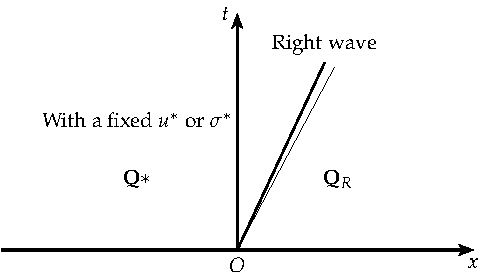
\includegraphics[width= 10cm] {Tikz-figure8.eps}
  \caption{Half Riemann problem  with a given left velocity or Cauchy stress..}
  \label{fig:half}
\end{figure}

As we know the velocity $u^*$ or the Cauchy stress $\sigma ^*$, there is only one function need to be solved as
\begin{equation}\label{eq:halfu}
  f(\rho^*,\mathbf{Q}_R) =u(\rho^*,\mathbf{Q}_R) - u^* = 0,
\end{equation}
or
\begin{equation}\label{eq:halfs}
  f(\rho^*,\mathbf{Q}_R) =\sigma(\rho^*,\mathbf{Q}_R) - \sigma^* = 0.
\end{equation}
Samilar to the process in Section (\ref{sec:iteration}), we have to use an iteration procedure to solve (\ref{exact1}) and
the solving process is list in the following.

\noindent  \textbf{Initial:}

	The initial density is  given as
\begin{equation}
\rho_{(0)}^* = \rho_R.
\end{equation}
\textbf{Iteration begin:}
\begin{enumerate}[Step 1]
  \item Case select:
	By a given  $\rho _{(k)}^*$ in $k$ iteration step, we need to determine the case of the wave structures in the left side. The determining  process is  also done in Section \ref{sec:deter}.

  \item Solving $f$:  After determining the structure case, we need to solve the velocity ( or  the Cauchy stress) in  the region $\mathbf{Q}^*$, this is  given in Section \ref{sec:functions}.

  \item  Updating   $\rho^*$:   By the Newton iteration equation, a new density can be updated as

\begin{equation}
 \rho^*_{(k+1)} = \rho^*_{(k)}- f/\frac{\partial f_{(k)}}{\partial \rho},
\end{equation}
The derivatives of $f$ is  given by
\begin{equation}
  \frac{\partial f_{(k+1)}}{\partial \rho^*} = \frac{f_{(k+1)}-f_{(k)}}{\rho_{(k+1)}^* - \rho^*_{(k)}},
\end{equation}
At the first step, we use a simple  numerical difference  method
\begin{equation}
  \frac{\partial f_{(1)}}{\partial \rho^*} = \frac{f(\rho^*+\Delta \rho)-f(\rho^*)}{\Delta \rho},
\end{equation}
where $\Delta \rho$ is a little quatity, we can choose it as
\begin{equation}
  \Delta \rho = \frac{\rho_{(0)}^*}{100}.
\end{equation}
\item Convergence test:
The  convergence is meassured by
\begin{equation}
\text{CHA} = \text{max} \left[
\frac{|\rho_{(k+1)}^*- \rho_{(k)}^*|}{\frac{1}{2}|\rho_{(k+1)}^*+\rho_{(k)}^*|},|f|\right].
\end{equation}
and the tolerance is taken as $\text{TOL} = 10^{-4}$.

If $ \text{CHA} \le \text{TOL} $, the iteration ends.
It usually takes 2-4 step to get a convergence result.
\end{enumerate}
\textbf{Iteration end.}
\section{Numerical  tests }
In this section, by choosing suitable initial conditions, we will solve the Riemann problem with several different structure cases in the solution. For simple  expression, in figures, we use same representations as those in \cite{gao2018complete}. ``$|$'' means the contact wave, and capital letters ''S'' and ''R'' means the shock and rarefaction wave. Superscript letters ''E'' and  ''P'' indicate the elastic or plastic state of a wave.  Numerical results by the method  in \cite{liumulti} is used to verified the correctness of the exact solution. In the following tests, the materials are taken as  aluminium and copper. The parameters for the EOS and constitutive model for aluminum and copper  are
$ (\rho_0, a_0, \Gamma_0, s, \mu)_{\text{Al}} =(8930 \text{kg}/\text{m}^3, 3940 \text{m}/\text{s},2, 1.49, 2.76 ,2.76\times 10^{10} \text{Pa} )$ and   $(\rho_0, a_0, \Gamma_0, s, \mu)_{\text{copper}} =(2785 \text{kg}/\text{m}^3, 5328 \text{m}/\text{s},2, 1.338,4.5\times 10^{10}\text{Pa})$, respectively. The computational domain is set to be $[0,1m]$ with 800 cell points and the intial interface is located at $0.5m$, the terminal time is $t=5\times 10^{-5}s$.

\subsection{Test 1}
In this case, the material is yielding at both sides, so the solution structure has three wave with two plastic waves and one contact.
The initial condition is
\begin{equation}
 \left\{ \begin{aligned}
&	 \text{L: Al,}\quad  \rho = 2785 \text{kg}/\text{m}^3, \quad  u = 20\text{m}/\text{s}, \quad  p = 1.0\text{Pa}, \quad  s_{xx}=-2.0\times 10^8 \text{Pa},\\
&	 \text{R: Al,}\quad  \rho = 2785 \text{kg}/\text{m}^3, \quad  u = 0\text{m}/\text{s}, \quad  p = 1.0\text{Pa}, \quad  s_{xx}=-2.0\times 10^8 \text{Pa},\\
   \end{aligned}
 \right.
\end{equation}
It can be seen that the exact solution matches the numerical results very well in Fig.\ref{fig:case1}.
\begin{figure}
  \centering

  %\includegraphics[width= 8cm] {case1rho.pdf}
  %\includegraphics[width= 8cm] {case1u.pdf}
  %\includegraphics[width= 8cm] {case1p.pdf}
  %\includegraphics[width= 8cm] {case1sigma.pdf}

    \caption{Comparison resutls for Test 1 with the structrures of $S^P|S^P$.  }
  \label{fig:case1}
\end{figure}
\subsection{Test 2}
Next, we consider a case with yielding process at both sides, so the result has five waves. The initial condition is
\begin{equation}
 \left\{ \begin{aligned}
	 &	 \text{L: Al,}\quad  \rho = 2785 \text{kg}/\text{m}^3, \quad  u = 800\text{m}/\text{s}, \quad  p = 1.0\text{Pa}, \quad  s_{xx}=0.0 \text{Pa},\\
&	 \text{R: Al,}\quad  \rho = 2785 \text{kg}/\text{m}^3, \quad  u = 0\text{m}/\text{s}, \quad  p = 1.0\text{Pa}, \quad  s_{xx}=0.0 \text{Pa},\\
   \end{aligned}
 \right.
\end{equation}
Shown in Fig.\ref{fig:case2}, the exact solution matches the numerical results well generally, besides the under-cooling effect performed in the numerical results, but it is not considered in the designing of the exact Riemann solver.
\begin{figure}
  \centering
  %\includegraphics[width= 8cm] {case2rho.pdf}
  %\includegraphics[width= 8cm] {case2u.pdf}
  %\includegraphics[width= 8cm] {case2p.pdf}
  %\includegraphics[width= 8cm] {case2sxx.pdf}
  \caption{Comparison resutls for Test 1 with the structrures of $S^ES^P|S^PS^E$.  }
  \label{fig:case2}
\end{figure}

\subsection{Test 3}
In this example, we test the elastic rarefaction waves case. In the structrues there  is one  elastic rarefaction wave on each side of the contace wave. The initial condition is given as
\begin{equation}
 \left\{ \begin{aligned}
	 &	 \text{L: Al,}\quad  \rho = 2785 \text{kg}/\text{m}^3, \quad  u = -2.0\text{m}/\text{s}, \quad  p = 1.0\time 10^7\text{Pa}, \quad  s_{xx}=0.0 \text{Pa},\\
	 &	 \text{R: Al,}\quad  \rho = 2785 \text{kg}/\text{m}^3, \quad  u = 2.0\text{m}/\text{s}, \quad  p = 1.0\times 10^7 \text{Pa}, \quad  s_{xx}=0.0 \text{Pa},\\
   \end{aligned}
 \right.
\end{equation}
We can see that the results of the exact solution match the numerical results very well.
%
%j\section*{Conclusions}
\begin{figure}
  \centering

 % \includegraphics[width= 8cm] {case4rho.pdf}
 % \includegraphics[width= 8cm] {case4u.pdf}
 % \includegraphics[width= 8cm] {case4p.pdf}
 % \includegraphics[width= 8cm] {case4sxx.pdf}

    \caption{Comparison resutls for Test 3 with the structrures of $R^E|R^E$.  }
  \label{fig:case3}
\end{figure}
\subsection{Test 4}
Then we test another example with both elastic and plastic rarefaction  waves on both sides. The initial condition is
\begin{equation}
 \left\{ \begin{aligned}
	 &	 \text{L: Al,}\quad  \rho = 2785 \text{kg}/\text{m}^3, \quad  u = -40\text{m}/\text{s}, \quad  p = 1.0\times 10^7 \text{Pa}, \quad  s_{xx}=0.0 \text{Pa},\\
	 &	 \text{R: Al,}\quad  \rho = 2785 \text{kg}/\text{m}^3, \quad  u = 40\text{m}/\text{s}, \quad  p = 1.0\times 10^7\text{Pa}, \quad  s_{xx}=0.0 \text{Pa}.\\
   \end{aligned}
 \right.
\end{equation}
Results are shown in Fig.\ref{fig:case4},  the results of the exact solver matches the numerical results very well.

\begin{figure}
  \centering

%  \includegraphics[width= 8cm] {case3rho.pdf}
%  \includegraphics[width= 8cm] {case3u.pdf}
%  \includegraphics[width= 8cm] {case3p.pdf}
%  \includegraphics[width= 8cm] {case3sxx.pdf}

    \caption{Comparison resutls for Test 4 with the structrures of $R^ER^P|R^PR^E$.  }
  \label{fig:case4}
\end{figure}
\subsection{Test 5}
All the above four tests have symmetrical wave  structrues, next we will test an example with different structrues on different sides. The initial condition is given as
\begin{equation}
 \left\{ \begin{aligned}
&	 \text{L: Al,}\quad  \rho = 2785 \text{kg}/\text{m}^3, \quad  u = 40\text{m}/\text{s}, \quad  p = 1.0\times 10^8\text{Pa}, \quad  s_{xx}=-2.0\times 10^8 \text{Pa},\\
&	 \text{R: Al,}\quad  \rho = 2785 \text{kg}/\text{m}^3, \quad  u = -40\text{m}/\text{s}, \quad  p = 1.0 \times 10^2 \text{Pa}, \quad  s_{xx}=0.0\text{Pa}.\\
   \end{aligned}
 \right.
\end{equation}
In the Fig.\ref{fig:case5} shown in both the numerical and exact solutions, there is one plastic shock on the left side and both the elastic and plastic shocks exist on the right.

\begin{figure}
  \centering

 % \includegraphics[width= 8cm] {case5rho.pdf}
 % \includegraphics[width= 8cm] {case5u.pdf}
 % \includegraphics[width= 8cm] {case5p.pdf}
 % \includegraphics[width= 8cm] {case5sxx.pdf}

    \caption{Comparison resutls for Test 5 with the structrures of $R^P|R^PR^E$.  }
  \label{fig:case5}
\end{figure}
\subsection{Test 6}
In this test, we consider an example with zero initial velocities on both sides, driving by the gradient of the pressure, there are rarefaction waves producted into the higher pressure side and shock waves generated into the lower pressure side. The initial condition is given as
\begin{equation}
 \left\{ \begin{aligned}
	 &	 \text{L: Al,}\quad  \rho = 2785 \text{kg}/\text{m}^3, \quad  u = 0.0\text{m}/\text{s}, \quad  p = 1.0\times 10^{10} \text{Pa}, \quad s_{xx}= 0.0 \text{Pa},\\
	 &	 \text{R: Al,}\quad  \rho = 2785 \text{kg}/\text{m}^3, \quad  u = 0.0\text{m}/\text{s}, \quad  p = 1.0 \times 10^2 \text{Pa}, \quad  s_{xx}=0.0\text{Pa}.\\
   \end{aligned}
 \right.
\end{equation}
Shown in Fig.\ref{fig:case9}, we can see there are two shocks in the right side and two rarefaction waves on the left side.
\begin{figure}
  \centering

 % \includegraphics[width= 8cm] {case9rho.pdf}
 % \includegraphics[width= 8cm] {case9u.pdf}
 % \includegraphics[width= 8cm] {case9p.pdf}
 % \includegraphics[width= 8cm] {case9sxx.pdf}

    \caption{Comparison resutls for Test 6 with the structrures of $R^ER^P|S^PS^E$.  }
  \label{fig:case9}
\end{figure}
\subsection{Test 7}
Now we will consider two multi-material tests with different materials on different sides. In this test, on the left side, a lighter material of aluminum with a velocity impacts to a heavier material of copper. The initial condition is given as
\begin{equation}
 \left\{ \begin{aligned}
	 &	 \text{L: Al,}\quad  \rho = 2785 \text{kg}/\text{m}^3, \quad  u = 40\text{m}/\text{s}, \quad  p = 0.1\text{Pa}, \quad  s_{xx}=0.0\text{Pa},\\
	 &	 \text{R: Copper,}\quad  \rho = 8930\text{kg}/\text{m}^3, \quad  u = 0.0\text{m}/\text{s}, \quad  p =0.1\text{Pa}, \quad  s_{xx}=0.0\text{Pa}.\\
   \end{aligned}
 \right.
\end{equation}
Show in the Fig.\ref{fig:case7}, there is a large jump of density at the material interface and  both elastic shock and plastic shock exist in each side of the interface. The exact Riemann solver can solve the Riemann problem with multi-materials very well comparing to the MHLLCEP approximate solver.

\begin{figure}
  \centering
 % \includegraphics[width= 8cm] {case6rho.pdf}
 % \includegraphics[width= 8cm] {case6u.pdf}
 % \includegraphics[width= 8cm] {case6p.pdf}
 % \includegraphics[width= 8cm] {case6sigma.pdf}

    \caption{Comparison results for Test 7 with structrures of $R^ER^P|R^PR^E$.  }
  \label{fig:case7}
\end{figure}

%In this paper,  the multi-material HLLC-type  approximate Riemann solver with both the elastic and plastic waves (MHLLCEP) is constructed for 1D elastic-plastic  flows with a hypo-elastic model and the von Mises yielding condition. During constructing the  MHLLCEP, we do not use the assumption in which the pressure is continuous across the contact wave and so describing and evaluating the plastic waves are  more accurate than that in the  HLLCE.  Based on the MHLLCEP,
%combining with the third-order ghost-cell reconstruction method and the third-order TVD-Runge-Kutta method in time, a high-order cell-centered Lagrangian scheme for 1D multi-material elastic flows is built. Verified by the numerical experiments, both the plastic waves and elastic waves can be resolved correctly, our scheme appears to be convergent, stable, essentially non-oscillatory and can reach third-order accuracy for smooth problems. Especially for multi-material elastic-plastic flows, the results solved by the scheme with HLLCE are with large errors, but our new scheme can eliminate these errors and leads to the reasonable numerical results.
%
%
\subsection{Test 8}
At last, we test another multi-materials case, in this test the initial condtion is given as
\begin{equation}
 \left\{ \begin{aligned}
	 &	 \text{L: Copper,}\quad  \rho = 8930 \text{kg}/\text{m}^3, \quad  u = 0.0\text{m}/\text{s}, \quad  p = 1.0\times 10^{10}\text{Pa}, \quad  s_{xx}=0.0 \text{Pa},\\
	 &	 \text{R: Al,}\quad  \rho = 2785 \text{kg}/\text{m}^3, \quad  u = 0\text{m}/\text{s}, \quad  p = 10.0 \text{Pa}, \quad  s_{xx}=0.0 \text{Pa}.\\
   \end{aligned}
 \right.
\end{equation}
Shown in Fig.\ref{fig:case8}, there are two rarefaction waves on the left side and two shocks on the right side, there is a discontinuity of pressure on the interface, and the Cauchy stress is continuous, which  meets with the theoretical analysis.
\begin{figure}
  \centering
 % \includegraphics[width= 8cm] {case8rho.pdf}
 % \includegraphics[width= 8cm] {case8u.pdf}
 % \includegraphics[width= 8cm] {case8p.pdf}
 % \includegraphics[width= 8cm] {case8sigma.pdf}

    \caption{Comparison results for Test 8 with the structrures of $R^ER^P|S^ES^P$.  }
  \label{fig:case8}
\end{figure}
\subsection{Test 9}
Then we give two tests of  half Riemann problem, the first is with a given left velocity $u^* = -20\text{m/s}$, and the right initial condition is
\begin{equation}
 \text{Copper,}\quad\rho = 8930\text{kg}/\text{m}^3, \quad  u = 0.0\text{m}/\text{s}, \quad  p =0.1\text{Pa}, \quad  s_{xx}=0.0\text{Pa}.
\end{equation}
In Fig.\ref{fig:case9}, comparason results are given by the exact half Riemann solver and the numerical method. We can see that the exact solver  can resolve both the elastic and plastic shock waves well.
\begin{figure}
  \centering
 % \includegraphics[width= 8cm] {case10rho.pdf}
 % \includegraphics[width= 8cm] {case10u.pdf}
 % \includegraphics[width= 8cm] {case10p.pdf}
 % \includegraphics[width= 8cm] {case10sxx.pdf}

    \caption{Comparison results for Test 9 with the structrures of $S^ES^P$.  }
  \label{fig:case9}
\end{figure}
\subsection{Test 10}
The second half Riemann case is with  a given left Cauchy stress $\sigma^* = 0 \text{Pa}$, and the right initial condition is
\begin{equation}
  \text{Copper,}\quad\rho = 8930\text{kg}/\text{m}^3, \quad  u = 0.0\text{m}/\text{s}, \quad  p =1.0\times 10^9 \text{Pa}, \quad  s_{xx}=0.0\text{Pa}.
\end{equation}
In Fig.\ref{fig:case10}, we give the results computed by the exact Riemann solver and the numerical simulation, shown in it, the exact solver can resolve the elastic and plastic rarefaction waves well.
\begin{figure}
  \centering
%  \includegraphics[width= 8cm] {case11rho.pdf}
%  \includegraphics[width= 8cm] {case11u.pdf}
%  \includegraphics[width= 8cm] {case11p.pdf}
%  \includegraphics[width= 8cm] {case11sigma.pdf}
    \caption{Comparison results for Test 10 with the structrures of $R^ER^P$.  }
  \label{fig:case10}
\end{figure}
\section{Results}
In this paper, we give a detailed analysis of the Riemann problem for one-dimensional  multi-material elastic-plastic flows with the  Mie-Gr\"uneisen EOS, hypo-elastic constitutive model and the von Mises' yielding condition.  Some useful results are found through the analysing:
\begin{enumerate}
	\item The sonic speed periods a significant jump when the material is yielding.
	\item the plastic wave is always faster than the elastic wave for the reason of the sonic speed jump.
	
	  \item There are only thirty-six possible cases of the structrues in the Riemann problem.
	\item All the variables after the wave can be written as functions of the density theoretically.
	\end{enumerate}
	  Then, based on the analysis, we have constructed exact Riemann solvers for  both the Riemann problem  and the half Riemann problem, separately. Tested by  a large number of examples, the exact Riemann solver is reasonable and matching  well with the numerical method for both  single material problems and multi-material Riemann problems.

\section*{Acknowledgement}r
This work was supported by NSFC(Grant No. 11672047) and Science Challenge Project (Grant No. TZ2016002).

\bibliography{mybibfile}
  \appendix
  \renewcommand{\appendixname}{Appendix~}

  \section{Gauss-Legendre  quadrature}
  In this paper, we use Gauss-Legendre quadrature to  take  numerical integrations. 
For a function $f(x)$,  the intergration from $-1$ to $1$ is given as
$$ 
  \int_{-1}^1 f(x)dx \approx \sum_{i=0}^n \omega_i f(x_i)
$$
$\omega_i$ is the weight, and $x_i$ is the integrating point.
For different orders they are listed in Table \ref{tab:coe}. 

\subsection{}
\begin{table}\label{tab:coe}
  \centering
  \caption{Coefficiences for Guass-Legendere quadrature}
  \begin{tabular}{cccc}
	\toprule
	Number of points, $n$ &  Order & Points, $x_i$ & Weights, $\omega_i$ \\
	\midrule
	1 & 1  & 0 & 2 \\
	\hline
	2 & 3  & $\pm \frac{1}{\sqrt{3}}$ & 1 \\
	\hline
	\multirow{2}{*}{3} &\multirow{2}{*}{3} & 0  & $\frac{8}{9}$ \\
	\cline{3-4}
	& & $\pm\sqrt{\frac{3}{5}}$ & $\frac{5}{9} $\\
	\hline
	\multirow{2}{*}{\makecell{4}} & \multirow{2}{*}{7}  & $\pm \sqrt{\frac{3}{7} -\frac{2}{7}\sqrt{\frac{6}{5}}}$  & $\frac{18+\sqrt{30}}{36}$ \\
	\cline{3-4}
  &  &  $\pm \sqrt{\frac{3}{7} +\frac{2}{7}\sqrt{\frac{6}{5}}}$  & $\frac{18-\sqrt{30}}{36}$ \\
  \bottomrule
\end{tabular}
\end{table}

\end{document}
